%%%% 1. DOCUMENTCLASS %%%%
%
% \documentclass[journal=tches,submission,notanonymous]{iacrtrans}
\documentclass[journal=tches,submission]{iacrtrans}
%%%% NOTES:
% - Change "journal=tosc" to "journal=tches" if needed
% - Change "submission" to "final" for final version
% - Add "notanonymous" to reveal authors
% - Add "spthm" for LNCS-like theorems

% No indentation
% \setlength{\parindent}{0px}

%%%% 2. PACKAGES %%%%
\usepackage{algorithm}
\usepackage{algpseudocode}
\usepackage{caption}
\usepackage{multirow}
\usepackage{tikz}
\usetikzlibrary{positioning}
% \usepackage[demo]{graphicx}

%%%% 3. AUTHOR, INSTITUTE %%%%
\author{
    Ganyu Xu\inst{1}
    \and Kalikinkar Mandal\inst{2}
    \and Guang Gong\inst{1}
}
\institute{
  University of Waterloo, Waterloo, Canada, \email{{g66xu,ggong}@uwaterloo.ca}
  \and
  University of New Brunswick, New Brunswick, Canada, \email{kmandal@unb.ca}
}
%%%% NOTES:
% - We need a city name for indexation purpose, even if it is redundant
%   (eg: University of Atlantis, Atlantis, Atlantis)
% - \inst{} can be omitted if there is a single institute,
%   or exactly one institute per author

% Custom commands
\newcommand{\pke}{\texttt{PKE}}
\newcommand{\keygen}{\texttt{KeyGen}}
\newcommand{\encrypt}{\texttt{Enc}}
\newcommand{\decrypt}{\texttt{Dec}}
\newcommand{\kem}{\texttt{KEM}}
\newcommand{\encap}{\texttt{Encap}}
\newcommand{\decap}{\texttt{Decap}}
\newcommand{\etm}{\texttt{EtM}}  % encrypt-then-mac
\newcommand{\mac}{\texttt{MAC}}
\newcommand{\sign}{\texttt{Sign}}
\newcommand{\verify}{\texttt{Verify}}
\newcommand{\pk}{\texttt{pk}}
\newcommand{\sk}{\texttt{sk}}
\newcommand{\pco}{\texttt{PCO}}
\newcommand{\cvo}{\texttt{CVO}}
\newcommand{\leftsample}{\stackrel{\$}{\leftarrow}}
\newcommand{\llbrack}{[\![}
\newcommand{\rrbrack}{]\!]}
\newcommand{\norm}[1]{\left\lvert #1 \right\rvert}
\newcommand{\adv}{\texttt{Adv}}
\newcommand{\fotplus}{\texttt{FOT+}}
\newcommand{\us}{\mu s}
\def\mlkemplus{\text{ML-KEM}^+}

%%%% 4. TITLE %%%%
\title{Faster generic IND-CCA secure KEM using encrypt-then-MAC}
%%%% NOTES:
% - If the title is too long, or includes special macro, please
%   provide a "running title" as optional argument: \title[Short]{Long}
% - You can provide an optional subtitle with \subtitle.

\begin{document}

\maketitle


%%%% 5. KEYWORDS %%%%
\keywords{
    Key encapsulation mechanism, 
    Message authentication code,
    Post-quantum cryptography,
    Lattice cryptography,
    Fujisaki-Okamoto transformation
}


%%%% 6. ABSTRACT %%%%
\begin{abstract}
    ML-KEM is a lattice-based IND-CCA secure key encapsulation mechanism (KEM) standardized by NIST in FIPS 203. ML-KEM achieves chosen-ciphertext security by applying the Fujisaki-Okamoto transformation to an IND-CPA secure public-key encryption (PKE) scheme. The Fujisaki-Okamoto transformation uses de-randomization and re-encryption to ensure ciphertext non-malleability, but because ML-KEM's underlying PKE encryption is significantly slower than the underlying PKE decryption, ML-KEM's decapsulation performance is dominated by re-encryption. In this paper, we propose an alternative generic IND-CCA secure KEM transformation, called ${\sf KEM}_{{\tt EtM}}$ that applies the encrypt-then-MAC mechanism to an OW-PCA secure PKE and an existentially unforgeable MAC. Compared to the Fujisaki-Okamoto transformation, our encrypt-then-MAC transformation replaces de-randomization and re-encryption with computing a MAC tag. 
    We instantiate our proposed KEM with the PKE sub-routines of ML-KEM and call it $\mlkemplus$. We then implement $\mlkemplus$ with a wide selection of MACs including Poly1305, GMAC, CMAC, and KMAC. At the cost of minimal increase in encapsulation CPU cycles (+1.8\%) and ciphertext size (+2.1\%), $\mlkemplus$ achieves a massive reduction of decapsulation CPU cycles (-72.2\%) compared to ML-KEM. Furthermore, we implement key exchange protocols and measure realistic network round trip times (RTTs), where $\mlkemplus$ reduces RTTs by 23.9\%-39.5\% compared to ML-KEM.
\end{abstract}

\section{Introduction}\label{sec:introduction}
A key encapsulation mechanism (KEM) \cite{DBLP:journals/iacr/Shoup01} is a cryptographic primitive that allows two parties to establish a shared secret over an insecure channel. The desired security standard for a KEM is called indistinguishability under chosen-ciphertext attack (IND-CCA). Intuitively speaking, IND-CCA security requires that no efficient adversary can distinguish a pseudorandom shared secret from a uniformly random bit string of equal length, even with access to a decapsulation oracle throughout the attack. However, building a provably IND-CCA secure KEM is tremendously difficult. Early attempts without formal proofs, such as RSA encryption defined in PKCS\#1 v1.5 \cite{DBLP:journals/rfc/rfc2313}, were later shown to be vulnerable to practical chosen-ciphertext attacks \cite{DBLP:conf/crypto/Bleichenbacher98}. In recent decades, the most viable approach has been to start with cryptographic primitives possessing weaker security properties, such as a public-key encryption (PKE) scheme with one-way security under chosen-plaintext attack (OW-CPA), then add steps to achieve \emph{ciphertext non-malleability} \cite{DBLP:conf/asiacrypt/BellareN00}. Some of the earliest proposals for generic IND-CCA secure constructions include OAEP \cite{DBLP:conf/eurocrypt/BellareR94}, Fujisaki-Okamoto transformation \cite{DBLP:conf/crypto/FujisakiO99}\cite{DBLP:journals/joc/FujisakiO13}, REACT \cite{DBLP:conf/ctrsa/OkamotoP01}, and GEM \cite{DBLP:conf/ctrsa/CoronHJPPT02}. Some other notable examples for constructing IND-CCA secure public-key cryptosystems in the standard model include the constructions of Naor and Yung \cite{naor1990public}, Cramer and Shoup \cite{cramer1998practical} and Canetti, Halevi and Katz \cite{CCA-IBE-EUROCRYPT2004}. The construction of Naor and Yung uses an IND-CPA secure PKE and a non-interactive zero-knowledge (NIZK) proof system. Canetti, Halevi and Katz \cite{CCA-IBE-EUROCRYPT2004} proposed a construction to build an IND-CCA secure PKE scheme from an IND-CPA secure IBE scheme and a one-time signature scheme.

On the other hand, chosen-ciphertext security is a solved problem in symmetric cryptography. It is well understood that, by combining an IND-CPA secure symmetric encryption scheme with an existentially unforgeable message authentication code (MAC) in a pattern called encrypt-then-MAC \cite{DBLP:conf/crypto/Krawczyk01}, one can build an authenticated encryption scheme \cite{DBLP:conf/asiacrypt/BellareN00} that achieves IND-CCA security. The encrypt-then-MAC (EtM) mechanism was standard in ISO 19772 \cite{international2009iso-encrypt-then-mac}. While this technique cannot be directly applied in the context of public-key cryptography due to the lack of a shared symmetric key between the two communicating parties, the concept of authenticating ciphertext using a MAC still has strong merits. Abdalla, Rogaway, and Bellare proposed DHIES (also known as ``Hashed ElGamal'')\cite{DBLP:journals/iacr/AbdallaBR99}\cite{DBLP:conf/ctrsa/AbdallaBR01}, a hybrid public-key encryption (HPKE) scheme whose IND-CCA security reduces to the Gap Diffie-Hellman assumption \cite{DBLP:conf/pkc/OkamotoP01} under the random oracle model. The technique behind DHIES is to derive both the shared secret and a symmetric MAC key by hashing a random PKE plaintext, encrypting the PKE plaintext, then authenticating the PKE ciphertext using the previously derived MAC key. When the Gap Diffie-Hellman assumption holds and the MAC is existentially unforgeable, no efficient adversary can recover the decryption of an unknown ciphertext even with access to a decryption oracle because it cannot produce a valid tag for such unknown ciphertext. 

\subsection{Contributions}
Our main contributions are threefold: \begin{itemize}
    \item {\bf New IND-CCA secure KEM construction using encrypt-then-MAC.} We propose a generic IND-CCA secure KEM transformation called the encrypt-then-MAC transformation and prove that the IND-CCA security of the encrypt-then-MAC transformation reduces tightly to the OW-PCA security of the underlying PKE and the existential unforgeability of the underlying MAC. In addition, we argue that the encrypt-then-MAC transformation can be instantiated with one-time MAC such as Poly1305 for further performance improvements.
    \item {\bf $\mlkemplus$: Efficient CCA-secure KEM based on ML-KEM.} We present $\mlkemplus$, an IND-CCA secure KEM constructed by applying the encrypt-then-MAC transformation to ML-KEM's underlying PKE sub-routines. Compared to ML-KEM, $\mlkemplus$ adds a small amount of performance penalty to the encapsulation routine and a small increase in ciphertext size, but replaces the expensive re-encryption step in decapsulation with computing a MAC tag, which yields substantial performance improvements.
    \item {\bf Performance evaluation and comparisons.} We implemented $\mlkemplus$ in C and compared its performance with ML-KEM in a variety of scenarios. Compared to ML-KEM, $\mlkemplus$ achieves 72.2\%-79.1\% reduction of CPU cycle count for decapsulation while only increasing encapsulation's CPU cycle count by 1.8\%-7.3\% and ciphertext size by 1.0\%-2.0\% (see Table \ref{tbl:cpu-cycles-summary}). We also implemented the Kyber key exchange protocols \cite{DBLP:conf/eurosp/BosDKLLSSSS18} with $\mlkemplus$ and measured the round trip time (RTT) in realistic network settings. Compared to ML-KEM, $\mlkemplus$ achieves 24\%-28\% reduction of round trip time in unauthenticated key exchange (KE), 29\%-35\% in unilaterally authenticated key exchange (UAKE), and 35\%-48\% reduction in mutually authenticated key exchange (AKE). See Table \ref{tbl:rtt-summary} for a summary of round trip times.
\end{itemize}

\begin{table}[h]
    \centering
    \footnotesize
    % \small

    % TODO: Poly1305 may not be suitable for 192/256 bit security level
    \begin{tabular}{|p{1.2cm}|p{2.1cm}|p{2.6cm}|p{2.7cm}|}
        \hline
        & $\mlkemplus$-512 \newline (Poly1305)
        & $\mlkemplus$-768 \newline (KMAC 192-bit tag)
        & $\mlkemplus$-1024 \newline (KMAC 256-bit tag)
        \\
        \hline
        Encap \newline (ccl/tick) 
        & 91155 \newline (???) 
        & 150929 \newline (???) 
        & 228357 \newline (???) 
        \\
        \hline
        Decap \newline (ccl/tick) 
        & ??? \newline (???) 
        & ??? \newline (???) 
        & ??? \newline (???) 
        \\
        \hline
        CT size \newline (bytes) 
        & ??? \newline (???) 
        & ??? \newline (???) 
        & ??? \newline (???) 
        \\
        \hline
    \end{tabular}

    % Alternate version
    % \begin{tabular}{|p{2.5cm}|p{1.4cm}|p{1.4cm}|p{1.4cm}|}
    %    \hline
    %    & Encap \newline (ccl/tick) 
    %    & Decap \newline (ccl/tick) 
    %    & CT size \newline (bytes) \\
    %    \hline
    %    $\mlkemplus$-512 \newline (Poly1305)
    %    & 93157 \newline (+1.8\%)
    %    & 33733 \newline (-72.2\%)
    %    & 784 \newline (+2.1\%) \\
    %    \hline
    %    $\mlkemplus$-512 \newline (GMAC)
    %    & 97369 \newline (+6.5\%)
    %    & 37725 \newline (-68.9\%)
    %    & 784 \newline (+2.1\%) \\
    %    \hline
    %    $\mlkemplus$-512 \newline (CMAC)
    %    & 99739 \newline (+9.0\%)
    %    & 40117 \newline (-66.9\%)
    %    & 784 \newline (+2.1\%) \\
    %    \hline
    %    $\mlkemplus$-512 \newline (KMAC-256)
    %    & 101009 \newline (+10.4\%)
    %    & 40741 \newline (-66.4\%)
    %    & 784 \newline (+2.1\%) \\
    %    \hline
    % \end{tabular}

    \caption{$\mlkemplus$ achieves large performance improvements in decapsulation at the cost of minimal penalty in encapsulation performance and ciphertext size}\label{tbl:cpu-cycles-summary}
\end{table}

\begin{table}[h]
    \centering
    \footnotesize
    % \small

    % TODO: Poly1305 might not be suitable for 192/256 bit security
    \begin{tabular}{|p{1.6cm}|p{1.49cm}|p{1.49cm}|p{1.49cm}|}
        \hline
        &  $\text{ML-KEM}^+$ \newline 512 
        &  $\text{ML-KEM}^+$ \newline 768 
        &  $\text{ML-KEM}^+$ \newline 1024 
        \\
        \hline
        KE RTT \newline ($\us$) 
        &  ??? \newline (???) 
        &  ??? \newline (???) 
        &  ??? \newline (???) 
        \\
        \hline
        UAKE RTT \newline ($\us$) 
        &  ??? \newline (???) 
        &  ??? \newline (???) 
        &  ??? \newline (???) 
        \\
        \hline
        AKE RTT \newline ($\us$) 
        &  ??? \newline (???) 
        &  ??? \newline (???) 
        &  ??? \newline (???) 
        \\
        \hline
    \end{tabular}

    % Alternate version
    % \begin{tabular}{|p{2.5cm}|p{1.4cm}|p{1.8cm}|p{1.8cm}|}
    %    \hline
    %    & KE RTT \newline ($\us$) 
    %    & UAKE RTT \newline ($\us$) 
    %    & AKE RTT \newline ($\us$) \\
    %    \hline
    %    $\mlkemplus$-512 \newline (Poly1305)
    %    & 70 \newline (-23.9\%)
    %    & 103 \newline (-29.0\%)
    %    & 133 \newline (-39.5\%) \\
    %    \hline
    %    $\mlkemplus$-512 \newline (GMAC)
    %    & 73 \newline (-20.7\%)
    %    & 106 \newline (-26.9\%)
    %    & 139 \newline (-36.8\%) \\
    %    \hline
    %    $\mlkemplus$-512 \newline (CMAC)
    %    & 75 \newline (-18.5\%)
    %    & 108 \newline (-25.5\%)
    %    & 143 \newline (-35.0\%) \\
    %    \hline
    %    $\mlkemplus$-512 \newline (KMAC-256)
    %    & 76 \newline (-17.4\%)
    %    & 109 \newline (-24.8\%)
    %    & 145 \newline (-34.1\%) \\
    %    \hline
    % \end{tabular}

    \caption{$\mlkemplus$ achieves substantial RTT savings despite increased encapsulation cost and ciphertext size}\label{tbl:rtt-summary}
\end{table}

\subsection{Related works}
\textbf{Optimal Asymmetric Encryption Padding (OAEP)} \cite{DBLP:conf/eurocrypt/BellareR94}\cite{DBLP:conf/crypto/BellareDPR98} is a generic chosen-ciphertext secure PKE. Under the random oracle model, the chosen-ciphertext security of the OAEP encryption scheme reduces to the one-wayness of the input trapdoor permutation. Although it was discovered that there exist trapdoor permutations with which the OAEP encryption scheme does not achieve full IND-CCA security \cite{DBLP:journals/joc/Shoup02}, Fujisaki et al. later proved that the OAEP is IND-CCA secure when combined with the RSA trapdoor permutation \cite{DBLP:conf/crypto/FujisakiOPS01}\cite{DBLP:journals/cacm/RivestSA78}. RSA-OAEP was standardized in PKCS\#1 v2 \cite{rfc8017} and is currently the most recommended of all RSA-based encryption schemes. Unfortunately, OAEP's requirement for a trapdoor permutation is immensely difficult to satisfy, and no other practical instantiation saw widespread adoption to this day.

The \textbf{Fujisaki-Okamoto transformation} \cite{DBLP:conf/crypto/FujisakiO99}\cite{DBLP:journals/joc/FujisakiO13} is another generic IND-CCA secure transformation. While Fujisaki and Okamoto originally proposed a hybrid public-key encryption scheme whose IND-CCA security reduces non-tightly to the OW-CPA security of the underlying PKE and the IND-CPA security of the symmetric encryption scheme. Later works \cite{DBLP:conf/ima/Dent03}\cite{DBLP:conf/tcc/HofheinzHK17}\cite{DBLP:conf/eurocrypt/DworkNR04}\cite{DBLP:conf/asiacrypt/HovelmannsHM22}\cite{bernstein2018towards}  tightened the security reduction, accounted for imperfect correctness, adapted the original proposal to build a KEM, and proved its security in the quantum random oracle model (QROM).

\begin{figure}[h]
    \centering

    \begin{minipage}[t]{0.34\textwidth}
        \begin{algorithm}[H]
            \caption*{$\kem^{\not\bot}_m.\keygen()$}
            \begin{algorithmic}[1]
                \State $(\pk, \sk^\prime) \leftsample \texttt{PKE.KeyGen}()$
                \State $z \leftsample \mathcal{M}$
                \State $\sk \leftarrow (\sk^\prime, \pk, z)$
                \State \Return $(\pk, \sk)$
            \end{algorithmic}
        \end{algorithm}
    \end{minipage}
    \begin{minipage}[t]{0.3\textwidth}
        \begin{algorithm}[H]
            \caption*{$\kem^{\not\bot}_m.\encap(\pk)$}
            \begin{algorithmic}[1]
                \State $m \leftsample \mathcal{M}$
                \State $r \leftarrow G(m)$
                \State $c \leftarrow \texttt{PKE.Enc}(\pk, m ,r)$
                \State $K \leftarrow H(m)$
                \State \Return $(c, K)$
            \end{algorithmic}
        \end{algorithm}
    \end{minipage}
    \begin{minipage}[t]{0.3\textwidth}
        \begin{algorithm}[H]
            \caption*{$\kem^{\not\bot}_m.\decap(\sk, c)$}
            \begin{algorithmic}[1]
                \State $\hat{m} \leftarrow \texttt{PKE.Dec}(\sk^\prime, c)$
                \State $\hat{r} \leftarrow G(m)$
                \State $\hat{c} \leftarrow \texttt{PKE.Enc}(\pk, \hat{m}, \hat{r})$
                \If{$\hat{c} = c$}
                    \State $K \leftarrow H(\hat{m})$
                \Else
                    \State $K \leftarrow H(z, c)$
                \EndIf
                \State \Return $K$
            \end{algorithmic}
        \end{algorithm}
    \end{minipage}

    \caption{The $\kem^{\not\bot}_m$ variant of Fujisaki-Okamoto transformation is used in ML-KEM}\label{fig:u-notbot-m-routines}
\end{figure}

The modular Fujisaki-Okamoto KEM transformation is remarkably successful because of the simplicity of its construction, the tightness of the security bound, and the proven (though non-tight) security against quantum adversaries. It was adopted by many submissions to NIST's post-quantum cryptography competition, including Kyber \cite{DBLP:conf/eurosp/BosDKLLSSSS18}, Saber \cite{DBLP:conf/africacrypt/DAnversKRV18}, FrodoKEM \cite{DBLP:conf/ccs/BosCDMNNRS16}, and classic McEliece \cite{classicmceliecespec} among others. The $U^{\not\bot}_m$ variant of the Fujisaki-Okamoto transformation (see Figure \ref{fig:u-notbot-m-routines}) is adopted in ML-KEM.

However, the Fujisaki-Okamoto transformation is not perfect. Because it uses re-encryption for achieving ciphertext non-malleability, the Fujisaki-Okamoto transformation suffers from the following two problems: \begin{itemize}
    \item \textbf{Computational inefficiency}. The decapsulation routine needs to re-encrypt the decryption to ensure ciphertext has not been tempered with. For input PKE whose encryption routine carries substantial computational cost, such as most lattice-based cryptosystems, re-encryption slows down decapsulation significantly.
    \item \textbf{Side-channel vulnerability}. Re-encryption also introduces side-channels that can leak information about the decrypted PKE plaintext. As demonstrated in \cite{ueno2022curse}\cite{ravi2019generic}\cite{DBLP:journals/tches/TanakaUXITH23}, these side-channels can be converted into efficient plaintext-checking attacks that can fully recover the secret key.
\end{itemize}

The rest of the paper is organized as follows. In Section \ref{sec:preliminaries}, we define and discuss the preliminary concepts and theorems. In Section \ref{sec:main-results}, we present our encrypt-then-MAC transformation in details, prove its security results, and discusses its relationship to the ElGamal cryptosystem. In Section \ref{sec:practical-instantiation-with-mlkem}, we present $\mlkemplus$, an instantiation of the encrypt-then-MAC transformation using ML-KEM's PKE sub-routines, then discuss some implementation rationales. In Section \ref{sec:performance-comparison}, we benchmark and compare the performance of individual KEM routines and key exchange round trip times between $\mlkemplus$ and ML-KEM.

\section{Preliminaries}\label{sec:preliminaries}

\subsection{Public-key encryption scheme}
\textbf{Syntax.} A public-key encryption scheme $\pke(\keygen, \encrypt, \decrypt)$ is a collection of three routines defined over some plaintext space $\mathcal{M}$ and some ciphertext space $\mathcal{C}$. Key generation $(\pk, \sk) \leftsample \keygen()$ is a randomized routine that returns a keypair. The encryption routine $\encrypt: (\pk, m) \mapsto c$ encrypts the input plaintext under the input public key. The decryption routine $\decrypt: (\sk, c) \mapsto m$ decrypts the input ciphertext under the input secret key. Where the encryption routine is randomized, we denote the randomness by a coin $r \in \mathcal{R}$, where $\mathcal{R}$ is called the coin space. The decryption routine is assumed to always be deterministic. Some decryption routines can detect malformed ciphertext and output the rejection symbol $\bot$ accordingly.

\textbf{Correctness.} Following the definition in \cite{DBLP:conf/eurocrypt/DworkNR04}, a $\pke$ is $\delta$-correct if:

\begin{equation*}
    E\left[\max_{m \in \mathcal{M}} P\left[\decrypt(\sk, c) \neq m \mid c \leftsample \encrypt(\pk, m)\right]\right] \leq \delta
\end{equation*}

Where the expectation is taken with respect to the probability distribution of all possible keypairs $(\pk, \sk) \leftsample \texttt{PKE.KeyGen()}$. For many lattice-based cryptosystems, including ML-KEM, decryption failures could leak information about the secret key, although the probability of a decryption failure is low enough that classical adversaries cannot exploit decryption failure more than they can defeat the underlying lattice problem.

\textbf{Security.} The security of public-key encryption is conventionally discussed within the context of adversarial games played between a challenger and an adversary \cite{DBLP:conf/stoc/GoldwasserM82}. There are two main types of games: in the one-wayness game, the adversary is given a random encryption, then asked to produce the correct decryption; in the indistinguishability game, the adversary is given the encryption of one of two adversary-chosen plaintexts, then asked to decide which of the plaintexts corresopnds with the given encryption. Depending on the attack model, the adversary may have access to various oracles. Within the context of public-key cryptography, adversaries are always assumed to have the public key with which they can mount chosen-plaintext attack (CPA). If the adversary has access to a plaintext-checking oracle (PCO) \cite{DBLP:conf/ctrsa/OkamotoP01} then it can mount plaintext-checking attack (PCA). Where the adversary has access to a decryption oracle, it can mount chosen-ciphertext attacks (CCA). 

\begin{figure}[H]
    \centering

    \begin{minipage}[t]{0.3\textwidth}
        \begin{algorithm}[H]
            \caption*{\texttt{OW-ATK} Game}
            \begin{algorithmic}[1]
                \State $(\pk, \sk) \leftsample \keygen(1^\lambda)$
                \State $m^\ast \leftsample \mathcal{M}$
                \State $c^\ast \leftsample \encrypt(\pk, m^\ast)$
                \State $\hat{m} \leftsample A^{\mathcal{O}_\texttt{ATK}}(1^\lambda, \pk, c^\ast)$
                \State \Return $\llbrack \hat{m} = m^\ast \rrbrack$
            \end{algorithmic}
        \end{algorithm}
    \end{minipage}
    \begin{minipage}[t]{0.33\textwidth}
        \begin{algorithm}[H]
            \caption*{\texttt{IND-ATK} Game}
            \begin{algorithmic}[1]
                \State $(\pk, \sk) \leftsample \keygen(1^\lambda)$
                \State $(m_0, m_1) \leftsample A^{\mathcal{O}_\texttt{ATK}}(1^\lambda, \pk)$
                \State $b \leftsample \{0,1\}$
                \State $c^\ast \leftsample \encrypt(\pk, m_b)$
                \State $\hat{b} \leftsample A^{\mathcal{O}_\texttt{ATK}}(1^\lambda, \pk, c^\ast)$
                \State \Return $\llbrack \hat{b} = b \rrbrack$
            \end{algorithmic}
        \end{algorithm}
    \end{minipage}
    \begin{minipage}[t]{0.33\textwidth}
        \begin{algorithm}[H]
            \caption*{$\mathcal{O}_\pco(m, c)$}
            \begin{algorithmic}[1]
                \State \Return $\llbrack m = \decrypt(\sk, c) \rrbrack$
            \end{algorithmic}
        \end{algorithm}
        \begin{algorithm}[H]
            \caption*{$\mathcal{O}_\decrypt(c)$}
            \begin{algorithmic}[1]
                \State \Return $\decrypt(\sk, c)$
            \end{algorithmic}
        \end{algorithm}
    \end{minipage}
    \caption{The one-way game, indistinguishability game, plaintext-checking oracle (PCO), and decryption oracle. $\texttt{ATK} \in \{\texttt{CPA}, \texttt{PCA}, \texttt{CCA}\}$}
\end{figure}

The advantage of an adversary in the \texttt{OW-ATK} game is the probability that it ouputs the correct decryption. The advantage of an adversary in the \texttt{IND-ATK} game is defined below. A PKE is \texttt{OW-ATK}/\texttt{IND-ATK} secure if no efficient adversary has non-negligible advantage in the corresponding security game.

\begin{equation*}
    \texttt{Adv}_\texttt{IND-ATK}(A) = \left\vert P\left[ \hat{b} = b \right] - \frac{1}{2} \right\vert
\end{equation*}

\subsection{Key encapsulation mechanism (KEM)}
\textbf{Syntax} A key encapsulation mechanism $\kem(\keygen, \encap, \decap)$ is a collection of three routines defined over some ciphertext space $\mathcal{C}$ and some key space $\mathcal{K}$. The key generation routine takes the security parameter $1^\lambda$ and outputs a keypair $(\pk, \sk) \leftsample \keygen(1^\lambda)$. $\encap(\pk)$ is a probabilistic routine that takes a public key $\pk$ and outputs a pair of values $(c, K)$ where $c \in \mathcal{C}$ is the ciphertext (also called encapsulation) and $K \in \mathcal{K}$ is the shared secret (also called session key). $\decap(\sk, c)$ is a deterministic routine that takes the secret key $\sk$ and the encapsulation $c$ and returns the shared secret $K$ if the ciphertext is valid. Some KEM constructions use explicit rejection, where if $c$ is invalid then $\decap$ will return a rejection symbol $\bot$; other KEM constructions use implicit rejection, where if $c$ is invalid then $\decap$ will return a fake session key that depends on the ciphertext and some other secret values.

\textbf{Security} The security of KEMs is similarly discussed in adversarial games (Figure \ref{fig:kem-game}), although the win conditions differ slightly from the win conditions of a PKE's indistinguishability game. In a KEM's indistinguishability game, an adversary is given the public key and a challenge ciphertext, then asked to distinguish a pseudorandom shared secret $K_0$ associated with the challenge ciphertext from a truly random bit string of equal length.

\begin{figure}[h]
    \centering
    \begin{minipage}[t]{0.49\textwidth}
        \begin{algorithm}[H]
            \caption*{\texttt{IND-ATK} game}
            \begin{algorithmic}[1]
                \State $(\pk, \sk) \leftsample \keygen(1^\lambda)$
                \State $(c^\ast, K_0) \leftsample \encap(\pk)$
                \State $K_1 \leftsample \mathcal{K}$
                \State $b \leftsample \{0, 1\}$
                \State $\hat{b} \leftsample A^{\mathcal{O}_\texttt{ATK}}(
                    1^\lambda, \pk, c^\ast, K_b
                )$
                \State \Return $\llbrack \hat{b} = b \rrbrack$
            \end{algorithmic}
        \end{algorithm}
    \end{minipage}\hfill
    \begin{minipage}[t]{0.49\textwidth}
        \begin{algorithm}[H]
        \caption*{$\mathcal{O}_\decap(c)$}
        \begin{algorithmic}[1]
            \State \Return $\decap(\sk, c)$
        \end{algorithmic}
        \end{algorithm}
    \end{minipage}
    \caption{\texttt{IND-ATK} game for KEM and decapsulation oracle $\mathcal{O}_\decap$}\label{fig:kem-game}
\end{figure}

The decapsulation oracle $\mathcal{O}^\decap$ takes a ciphertext $c$ and returns the output of the $\decap$ routine using the secret key. The advantage $\epsilon_\texttt{IND-CCA}$ of an IND-CCA adversary $\mathcal{A}_\texttt{IND-CCA}$ is defined by the adversary's ability to correctly distinguish the two cases beyond blind guess:

\begin{equation*}
    \adv_\texttt{IND-CCA}(A) = \norm{
        P[A^{\mathcal{O}_\decap}(a^\lambda, \pk, c^\ast, K_b) = b] - \frac{1}{2}
    }
\end{equation*}

A KEM is \texttt{IND-ATK} secure if no efficient adversary has non-negligible advantage in the corresponding security game.

\subsection{Message authentication code (MAC)}\label{sec:message-authentication-code}
A message authentication code $\mac(\keygen, \sign, \verify)$ is a collection of routines defined over some key space $\mathcal{K}$, some message space $\mathcal{M}$, and some tag space $\mathcal{T}$. The signing routine $\sign(k, m)$ authenticates the message $m$ under the secret key $k$ by producing a tag $t$ (also called digest). The verification routine $\verify(k, m, t)$ takes the triplet of secret key, message, and tag, and outputs $\texttt{1}$ if the message-tag pair is valid under the secret key, or $\texttt{0}$ otherwise. Many MAC constructions are deterministic. For these constructions it is simpler to denote the signing routine by $t \leftarrow \mac(k, m)$ and perform verification using a simple comparison.

The security of a MAC is defined in an adversarial game in which an adversary, with access to some signing oracle $\mathcal{O}_\sign(m)$, tries to forge a new valid message-tag pair that has never been queried before. The existential unforgeability under chosen message attack (EUF-CMA) game is shown below:

\begin{figure}[H]
    \centering
    \begin{minipage}{0.53\textwidth}
        \begin{algorithm}[H]
            \caption*{\texttt{EUF-CMA} game}
            \begin{algorithmic}[1]
                \State $k^\ast \leftsample \mathcal{K}$
                \State $(\hat{m}, \hat{t}) \leftsample \mathcal{A}^{\mathcal{O}_\sign}()$
                \State \Return $
                    \llbrack \verify(k^\ast, \hat{m}, \hat{t}) 
                    \land (\hat{m}, \hat{t}) \not\in \mathcal{O}_\sign
                    \rrbrack
                $
            \end{algorithmic}
        \end{algorithm}
    \end{minipage}
    \caption{The existential forgery game}\label{fig:euf-cma-game}
\end{figure}

The advantage $\adv_\texttt{EUF-CMA}$ of the existential forgery adversary is the probability that it wins the EUF-CMA game. Some MACs are one-time existentially unforgeable, meaning that each secret key can be used to authenticate only a single message. The corresponding security game is modified such that the signing oracle will only answer a single signing query.

\section{The encrypt-then-MAC transformation}\label{sec:main-results}
In this section we introduce the encrypt-then-MAC transformation that transforms an OW-PCA secure PKE and an one-time existentially unforgeable MAC into an IND-CCA secure KEM. Our scheme mainly differs from DHIES in its versatility and input requirement. Whereas the IND-CCA security of DHIES reduces specifically to the Gap Diffie-Hellman assumption, the chosen-ciphertext security of the encrypt-then-MAC KEM reduces more generally to the OW-PCA security \cite{DBLP:conf/ctrsa/OkamotoP01} of the input scheme (we will show in Section \ref{sec:elgamal-is-ow-pca} that the Gap Diffie-Hellman assumption implies OW-PCA security). In addition, we propose that because each call to encapsulation samples a fresh PKE plaintext, the encrypt-then-MAC KEM can be instantiated with one-time secure MAC such as Poly1305 for further performance improvements (M. Abdalla et al. originally proposed to use HMAC and CBC-MAC, which are many-time secure MAC but less efficient than one-time MAC, see Section \ref{sec:choosing-a-message-authenticator}). The encapsulation data flow is illustrated in Figure \ref{fig:etm-diagram}.

\begin{figure}[h]
    \centering
    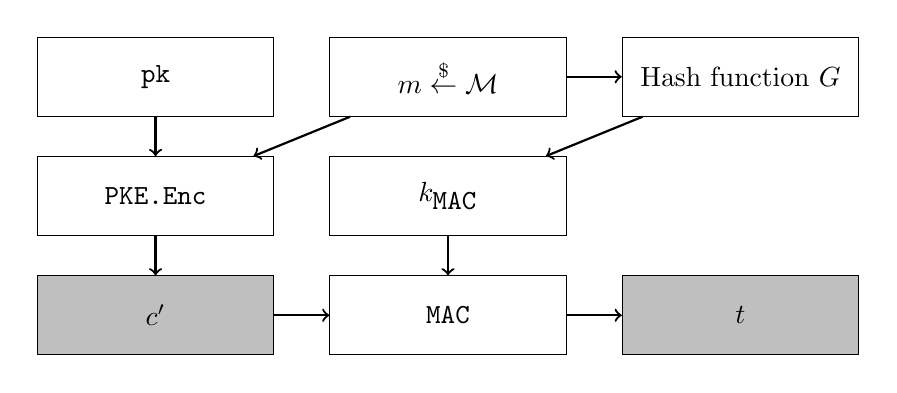
\begin{tikzpicture}
        \tikzstyle{rect} = [draw, rectangle, minimum width=3cm, minimum height=1cm]
        \tikzstyle{filledrect} = [draw, rectangle, minimum width=3cm, minimum height=1cm, fill=lightgray]
        \matrix [column sep=7mm, row sep=5mm] {
            \node (pk) [rect] {$\pk$}; &
            \node (m) [rect] {$m \leftsample \mathcal{M}$}; &
            \node (hashg) [rect] {Hash function $G$}; \\
            \node (pkeenc) [rect] {$\texttt{PKE.Enc}$}; &
            \node (mackey) [rect] {$k_\mac$}; \\
            \node (ct) [filledrect] {$c^\prime$}; &
            \node (mac) [rect] {$\mac$}; &
            \node (tag) [filledrect] {$t$}; \\
        };
        \draw[->, thick] (pk) -- (pkeenc);
        \draw[->, thick] (m) -- (pkeenc);
        \draw[->, thick] (m) -- (hashg);
        \draw[->, thick] (hashg) -- (mackey);
        \draw[->, thick] (pkeenc) -- (ct);
        \draw[->, thick] (mackey) -- (mac);
        \draw[->, thick] (ct) -- (mac);
        \draw[->, thick] (mac) -- (tag);
    \end{tikzpicture}

    \caption{Combining PKE with MAC using encrypt-then-MAC to ensure ciphertext integrity}\label{fig:etm-diagram}
\end{figure}

In Section \ref{sec:proof-of-theorem} we reduce the IND-CCA security of the KEM tightly to the OW-PCA security of the underlying PKE, and non-tightly to the unforgeability of the MAC. In Section \ref{sec:elgamal-is-ow-pca}, we show that DHIES is a special case of the encrypt-then-MAC transformation by reducing the OW-PCA security of the ElGamal cryptosystem to the Gap Diffie-Hellman assumption.

Let $\mathcal{B}^\ast$ denote the set of finite bit strings. Let $\pke(\keygen, \encrypt, \decrypt)$ be a public-key encryption scheme defined over message space $\mathcal{M}$ and ciphertext space $\mathcal{C}$. Let $\mac: \mathcal{K}_\mac \times \mathcal{B}^\ast \rightarrow \mathcal{T}$ be a deterministic message authentication code that takes a key $k \in \mathcal{K}_\mac$, some message $m \in \mathcal{B}^\ast$, and outputs a digest $t \in \mathcal{T}$. Let $G: \mathcal{M} \rightarrow \mathcal{K}_\mac$ be a hash function that maps from $\pke$'s plaintext space to $\mac$'s key space. Let $H: \mathcal{B}^\ast \rightarrow \mathcal{K}_\kem$ be a hash function that maps bit strings into the set of possible shared secrets. The encrypt-then-MAC transformation $\etm[\pke, \mac, G, H]$ constructs a key encapsulation mechanism $\kem_\etm(\keygen, \encap, \decap)$, whose routines are described in Figure \ref{fig:etm-routines}.

\begin{figure}[h]
    \centering
    \begin{minipage}[t]{0.5\textwidth}
        \begin{algorithm}[H]
            \caption*{$\kem_\etm.\keygen()$}
            \begin{algorithmic}[1]
                \State $(\pk, \sk^\prime) \leftsample \pke\texttt{.}\keygen()$
                \State $z \leftsample \mathcal{M}$
                \State $\sk \leftarrow (\sk^\prime, z)$
                \State \Return $(\pk, \sk)$
            \end{algorithmic}
        \end{algorithm}
        \begin{algorithm}[H]
            \caption*{$\kem_\etm.\encap(\pk)$}
            \begin{algorithmic}[1]
                \State $m \leftsample \mathcal{M}$
                \State $k \leftarrow G(m)$
                \State $c^\prime \leftsample \pke\texttt{.}\encrypt(\pk, m)$
                \State $t \leftarrow \mac(k, c^\prime)$
                \State $c \leftarrow (c^\prime, t)$
                \State $K \leftarrow H(m, c)$
                \State \Return $(c, K)$
            \end{algorithmic}
        \end{algorithm}
    \end{minipage}\hfill
    \begin{minipage}[t]{0.49\textwidth}
        \begin{algorithm}[H]
            \caption*{$\kem_\etm.\decap(\sk, c)$}
            \begin{algorithmic}[1]
                \State $(c^\prime, t) \leftarrow c$
                \State $(\sk^\prime, z) \leftarrow \sk$
                \State $\hat{m} \leftarrow \pke\texttt{.}\decrypt(\sk^\prime, c^\prime)$
                \State $\hat{k} \leftarrow G(\hat{m})$
                \If{$\mac(\hat{k}, c^\prime) = t$}
                    \State $K \leftarrow H(\hat{m}, c)$
                \Else
                    % This is directly copied from ML-KEM, DO NOT CHANGE
                    \State $K \leftarrow H(z, c)$
                \EndIf
                \State \Return $K$
            \end{algorithmic}
        \end{algorithm}
    \end{minipage}
    \caption{The encrypt-then-MAC transformation builds a KEM $\kem_\etm$ using a $\pke(\keygen, \encrypt, \decrypt)$, a $\mac$, and two hash functions $G, H$}\label{fig:etm-routines} 
\end{figure}

The key generation routine of $\kem_\etm$ is largely identical to that of the $\pke$, only a secret value $z$ is sampled as the implicit rejection symbol. In the encapsulation routine, a MAC key is derived from the randomly sampled plaintext, then used to sign the unauthenticated ciphertext $c^\prime$. Finally, the unauthenticated ciphertext $c^\prime$ and the tag $t$ combine into the authenticated ciphertext $c$ that would be transmitted to the peer. In the decapsulation routine, the decryption $\hat{m}$ of the unauthenticated ciphertext is used to re-derive the MAC key $\hat{k}$, which is then used to re-compute the tag $\hat{t}$. The ciphertext is considered valid if and only if the recomputed tag is identical to the input tag.

% Here are some additional design rationales that have practical impact on security and performance but do not affect the security proof: \begin{itemize}
%     \item \textbf{Removing de-randomization.} Since the encrypt-then-MAC transformation removes re-encryption in decapsulation, there is no longer the need for fixing the pseudorandom coin $r$ in the PKE's encryption routine. If the input PKE is already rigid, then the shared secret may be derived from hashing the PKE plaintext alone. However, if the input PKE is not rigid, then the shared secret must be derived from hashing both the PKE plaintext and the PKE ciphertext. 
%     \item \textbf{Hashing the public key.} The public key goes into deriving both the MAC key and the shared secret for two main reasons. First, in a realistic key exchange, the public key and the random PKE plaintext are generated by opposite parties. Hashing both the public key and the PKE plaintext ensures that both parties have inputs into the shared secret. Second, if the MAC key is derived from the PKE plaintext alone, then an adversary can pre-compute a large dictionary mapping MAC keys to the pre-image PKE plaintext. Upon receiving some ciphertext, an adversary can search through this key-plaintext dictionary and recover the decryption. Adding the public key into the derivation of the MAC key will dramatically increase the space and time requirement of such dictionary attack and render it infeasible in practice.
%     \item \textbf{Hashing the MAC tag instead of the entire ciphertext.} Because we allow the PKE to be randomized, the shared secret must have inputs from both the plaintext and the ciphertext. However, we find it unnecessary to hash the entire ciphertext. Instead, since the MAC tag functions as a keyed hash of the ciphertext, we can use the MAC tag as a substitute ciphertext hash, which yields meaningful performance improvements for shared secret derivation. On the other hand, not hashing the entire ciphertext will not give an adversary additional advantage because asssuming that the adversary does not already know the underlying decryption, it cannot tamper with any part of the challenge ciphertext without making the ciphertext-tag invalid, so the decapsulation oracle will always return the implicit rejection.
% \end{itemize}

The chosen-ciphertext security of the encrypt-then-MAC scheme can be intuitively argued through an adversary's inability to learn additional information from the decapsulation oracle. For an adversary $A$ to produce a valid tag $t$ for some unauthenticated ciphertext $c^\prime$ under the symmetric key $k \leftarrow G(\decrypt(\sk^\prime, c^\prime))$ implies that $A$ must either know the symmetric key $k$ or produce a forgery. Under the random oracle model, $A$ also cannot know $k$ without knowing its preimage $\decrypt(\sk^\prime, c^\prime)$, so $A$ must either have produced $c^\prime$ honestly, or have broken the one-way security of $\pke$. This means that the decapsulation oracle will not give out information on decryptions that the adversary does not already know. 

However, a decapsulation oracle can still give out some information: for a known plaintext $m$, all possible encryptions $c^\prime \leftsample \encrypt(\pk, m)$ can be correctly signed, while ciphertexts that don't decrypt back to $m$ cannot be correctly signed. This means that a decapsulation oracle can be converted into a plaintext-checking oracle, so every chosen-ciphertext attack against the KEM can be converted into a plaintext-checking attack against the underlying PKE.

On the other hand, if the underlying PKE is OW-PCA secure and the underlying MAC is one-time existentially unforgeable, then the encrypt-then-MAC KEM is IND-CCA secure:

\begin{theorem}\label{thm:ow-pca-implies-kem-ind-cca2}
    For every \texttt{IND-CCA} adversary $A$ against $\kem_\etm$ that makes $q$ decapsulation queries, there exists an \texttt{OW-PCA} adversary $B$ who makes at least $q$ plaintext-checking queries against the underlying $\pke$, and an one-time existential forgery adversary $C$ against the underlying $\mac$ such that

    \begin{equation*}
        \texttt{Adv}_\texttt{IND-CCA}(A) \leq q \cdot \adv_\texttt{OT-MAC}(C) + 2 \cdot \texttt{Adv}_\texttt{OW-PCA}(B)
    \end{equation*}
\end{theorem}

Theorem \ref{thm:ow-pca-implies-kem-ind-cca2} naturally flows into an equivalence relationship between the security of the KEM and the security of the PKE:

\begin{lemma}
    $\kem_\etm$ is IND-CCA secure if and only if the input $\pke$ is OW-PCA secure
\end{lemma}

\subsection{Proof of theorem \ref{thm:ow-pca-implies-kem-ind-cca2}}\label{sec:proof-of-theorem}
We will prove Theorem \ref{thm:ow-pca-implies-kem-ind-cca2} using a sequence of game. A summary of the the sequence of games can be found in Figure \ref{fig:etm-ind-cc2-sequence-of-games} and \ref{fig:ow-pca-simulates-game-3}. From a high level we made three incremental modifications to the IND-CCA game for $\kem_\etm$: replace true decapsulation with simulated decapsulation, replace the pseudorandom MAC key $k^\ast \leftarrow G(\pk, m^\ast)$ with a truly random MAC key $k^\ast \leftsample \mathcal{K}_\mac$, and finally replace pseudorandom shared secret $K_0 \leftarrow H(m^\ast, t)$ with a truly random shared secret $K_0 \leftsample \mathcal{K}_\kem$. A OW-PCA adversary can then simulate the modified IND-CCA game for the KEM adversary, and the advantage of the OW-PCA adversary is associated with the probability of certain behaviors of the KEM adversary.

\begin{figure}[h]
    \centering
    \begin{minipage}[t]{0.5\textwidth}
        \begin{algorithm}[H]
            \caption*{\texttt{IND-CCA} game for $\kem_\etm$}
            \begin{algorithmic}[1]
                \State $(\pk, \sk) \leftsample \kem_\etm\texttt{.}\keygen()$
                \State $m^\ast \leftsample \mathcal{M}$
                \State $c^\prime \leftsample \pke\texttt{.}\encrypt(\pk, m^\ast)$
                \State $k^\ast \leftarrow G(m^\ast)$
                    \Comment{Game 0-1}
                \State $k^\ast \leftsample \mathcal{K}_\mac$
                    \Comment{Game 2-3}
                \State $t \leftarrow \mac(k^\ast, c^\prime)$
                \State $c^\ast \leftarrow (c^\prime, t)$
                \State $K_0 \leftarrow H(m^\ast, c^\ast)$
                    \Comment{Game 0-2}
                \State $K_0 \leftsample \mathcal{K}_\kem$
                    \Comment{Game 3}
                \State $K_1 \leftsample \mathcal{K}_\kem$
                \State $b \leftsample \{0,1\}$
                \State $\hat{b} \leftarrow A^{\mathcal{O}^\decap}(\pk, c^\ast, K_b)$
                    \Comment{Game 0}
                \State $\hat{b} \leftarrow A^{\mathcal{O}^\decap_1}(\pk, c^\ast, K_b)$
                    \Comment{Game 1-3}
                \State \Return $\llbrack \hat{b} = b \rrbrack$
            \end{algorithmic}
        \end{algorithm}
        \begin{algorithm}[H]
            \caption*{Hash oracle $\mathcal{O}^G(m)$}
            \begin{algorithmic}[1]
                \If{$\exists (\tilde{m}, \tilde{k}) \in \mathcal{L}^G : \tilde{m} = m$}
                    \State \Return $\tilde{k}$
                \EndIf
                \State $k \leftsample \mathcal{K}_\mac$
                \State $\mathcal{L}^G \leftarrow \mathcal{L}^G \cup \{(m, k)\}$
                \State \Return $k$
            \end{algorithmic}
        \end{algorithm}
    \end{minipage}
    \begin{minipage}[t]{0.49\textwidth}
        \begin{algorithm}[H]
            \caption*{Decap oracle $\mathcal{O}^\decap(c)$}
            \begin{algorithmic}[1]
                \State $(c^\prime, t) \leftarrow c$
                \State $\hat{m} = \decrypt(\sk^\prime, c^\prime)$
                \State $\hat{k} \leftarrow G(\hat{m})$
                \If{$\mac(\hat{k}, c^\prime) = t$}
                    \State $K \leftarrow H(\hat{m}, c)$
                \Else 
                    \State $K \leftarrow H(z, c)$
                \EndIf 
                \State \Return $K$
            \end{algorithmic}
        \end{algorithm}
        \vspace{-0.5cm}
        \begin{algorithm}[H]
            \caption*{$\mathcal{O}^\decap_1(c)$}
            \begin{algorithmic}[1]
                \State $(c^\prime, t) \leftarrow c$
                \If{$\exists (\tilde{m}, \tilde{k}) \in \mathcal{L}^G : 
                    \tilde{m} = \decrypt(\sk^\prime, c^\prime)
                    \land \mac(\tilde{k}, c^\prime) = t
                $}
                    \State $K \leftarrow H(\tilde{m}, c)$
                \Else
                    \State $K \leftarrow H(z, c)$
                \EndIf
                \State \Return $K$
            \end{algorithmic}
        \end{algorithm}
        \vspace{-0.5cm}
        \begin{algorithm}[H]
            \caption*{$\mathcal{O}^H(m, c)$}
            \begin{algorithmic}[1]
                \If{$\exists (\tilde{m}, \tilde{c}, \tilde{K}) \in \mathcal{L}^H : \tilde{m} = m \land \tilde{c} = c$}
                    \State \Return $\tilde{K}$
                \EndIf
                \State $K \leftsample \mathcal{K}_\kem$
                \State $\mathcal{L}^H \leftarrow \mathcal{L}^H \cup \{(m, c, K)\}$
                \State \Return $K$
            \end{algorithmic}
        \end{algorithm}
    \end{minipage}
    \caption{Sequence of games}\label{fig:etm-ind-cc2-sequence-of-games}
\end{figure}

\begin{proof}
    \emph{Game 0} is the standard IND-CCA game for KEMs. The decapsulation oracle $\mathcal{O}^\decap$ executes the decapsulation routine using the challenge keypair and return the results faithfully. The queries made to the hash oracles $\mathcal{O}^G, \mathcal{O}^H$ are recorded to their respective tapes $\mathcal{L}^G, \mathcal{L}^H$.

    \emph{Game 1} is identical to game 0 except that the true decapsulation oracle $\mathcal{O}^\decap$ is replaced with a simulated oracle $\mathcal{O}^\decap_1$. Instead of directly decrypting $c^\prime$ as in the decapsulation routine, the simulated oracle searches through the tape $\mathcal{L}^G$ to find a matching query $(\tilde{m}, \tilde{k})$ such that $\tilde{m}$ is the decryption of $c^\prime$. The simulated oracle then uses $\tilde{k}$ to validate the tag $t$ against $c^\prime$.

    If the simulated oracle accepts the queried ciphertext as valid, then there is a matching query that also validates the tag, which means that the queried ciphertext is honestly generated. Therefore, the true oracle must also accept the queried ciphertext. On the other hand, if the true oracle rejects the queried ciphertext, then the tag is simply invalid under the MAC key $k = G(\decrypt(\sk^\prime, c^\prime))$. Therefore, there could not have been a matching query that also validates the tag, and the simulated oracle must also rejects the queried ciphertext.

    This means that from the adversary $A$'s perspective, game 1 and game 0 differ only when the true oracle accepts while the simulated oracle rejects, which means that $t$ is a valid tag for $c^\prime$ under $k = G(\decrypt(\sk^\prime, c^\prime))$, but $k$ has never been queried. Under the random oracle model, such $k$ is a uniformly random sample of $\mathcal{K}_\mac$ that the adversary does not know, so for $A$ to produce a valid tag is to produce a forgery against the $\mac$ under an unknown and uniformly random key. Furthermore, the security game does not include a signing oracle, so this is a zero-time forgery. While zero-time forgery is not a standard security definition for a MAC, we can bound it by the advantage of a one-time forgery adversary $C$:

    \begin{equation*}
        P\left[\mathcal{O}^\decap(c) \neq \mathcal{O}^\decap_1(c)\right]
        \leq \adv_\texttt{OT-MAC}(C)
    \end{equation*}

    Across all $q$ decapsulation queries, the probability that at least one query is a forgery is thus at most $q \cdot P\left[\mathcal{O}^\decap(c) \neq \mathcal{O}^\decap_1(c)\right]$. By the difference lemma:

    \begin{equation*}
        \adv_{G_0}(A) - \adv_{G_1}(A) \leq q\cdot  \adv_\texttt{OT-MAC}(C)
    \end{equation*}

    \emph{Game 2} is identical to game 1, except that the challenger samples a uniformly random MAC key $k^\ast \leftsample \mathcal{K}_\mac$ instead of deriving it from $m^\ast$. From $A$'s perspective the two games are indistinguishable, unless $A$ queries $G$ with the value of $m^\ast$. Denote the probability that $A$ queries $G$ with $m^\ast$ by $P[\texttt{QUERY G}]$, then:

    \begin{equation*}
        \adv_{G_1}(A) - \adv_{G_2}(A) \leq P\left[\texttt{QUERY G}\right]
    \end{equation*}

    \emph{Game 3} is identical to game 2, except that the challenger samples a uniformly random shared secret $K_0 \leftsample \mathcal{K}_\kem$ instead of deriving it from $m^\ast$ and $t$. From $A$'s perspective the two games are indistinguishable, unless $A$ queries $H$ with $(m^\ast, \cdot)$. Denote the probability that $A$ queries $H$ with $(m^\ast, \cdot)$ by $P[\texttt{QUERY H}]$, then:

    \begin{equation*}
        \adv_{G_2}(A) - \adv_{G_3}(A) \leq P\left[\texttt{QUERY H}\right]
    \end{equation*}

    Since in game 3, both $K_0$ and $K_1$ are uniformly random and independent of all other variables, no adversary can have any advantage: $\adv_{G_3}(A) = 0$.

    \begin{figure}[h]
        \begin{minipage}[t]{0.49\textwidth}
            \begin{algorithm}[H]
                \caption*{$B(\pk, {c^\prime}^\ast)$}
                \begin{algorithmic}[1]
                    \State $z \leftsample \mathcal{M}$
                    \State $k \leftsample \mathcal{K}_\mac$
                    \State $t \leftarrow \mac(k, {c^\prime}^\ast)$
                    \State $c^\ast \leftarrow ({c^\prime}^\ast, t)$
                    \State $K \leftsample \mathcal{K}_\kem$
                    \State $\hat{b} \leftarrow A^{
                        \mathcal{O}^\decap_B, \mathcal{O}^G_B, \mathcal{O}^H_B
                    }(\pk, c^\ast, K)$
                    \If{$\texttt{ABORT}(m)$}
                        \State \Return $m$
                    \EndIf
                \end{algorithmic}
            \end{algorithm}
            \begin{algorithm}[H]
                \caption*{$\mathcal{O}^H_B(m, c)$}
                \begin{algorithmic}
                    \If{$\pco(m, {c^\prime}^\ast) = 1$}
                        \State $\texttt{ABORT}(m)$
                    \EndIf
                    \If{$
                        \exists (\tilde{m}, \tilde{c}, \tilde{K}) \in \mathcal{L}^H 
                        : \tilde{m} = m \land \tilde{c} = c
                    $}
                        \State \Return $\tilde{K}$
                    \EndIf
                    \State $K \leftsample \mathcal{K}_\kem$
                    \State $\mathcal{L}^H \leftarrow \mathcal{L}^H \cup \{(m, c, K)\}$
                    \State \Return $K$
                \end{algorithmic}
            \end{algorithm}
        \end{minipage}\hfill
        \begin{minipage}[t]{0.49\textwidth}
            \begin{algorithm}[H]
                \caption*{$\mathcal{O}^\decap_B(c)$}
                \begin{algorithmic}[1]
                    \State $(c^\prime, t) \leftarrow c$
                    \If{$\exists (\tilde{m}, \tilde{k}) \in \mathcal{L}^G : 
                        % \tilde{m} = \decrypt(\sk^\prime, c^\prime)
                        \pco(\tilde{m}, c^\prime) = 1
                        \land \mac(\tilde{k}, c^\prime) = t
                    $}
                        \State $K \leftarrow H(\tilde{m}, c)$
                    \Else
                        \State $K \leftarrow H(z, c)$
                    \EndIf
                    \State \Return $K$
                \end{algorithmic}
            \end{algorithm}
            \begin{algorithm}[H]
                \caption*{$\mathcal{O}^G_B(m)$}
                \begin{algorithmic}[1]
                    \If{$\pco(m, {c^\prime}^\ast) = 1$}
                        \State $\texttt{ABORT}(m)$
                    \EndIf
                    \If{$\exists (\tilde{m}, \tilde{k}) \in \mathcal{L}^G : \tilde{m} = m$}
                        \State \Return $\tilde{k}$
                    \EndIf
                    \State $k \leftsample \mathcal{K}_\mac$
                    \State $\mathcal{L}^G \leftarrow \mathcal{L}^G \cup \{(m, k)\}$
                    \State \Return $k$
                \end{algorithmic}
            \end{algorithm}
        \end{minipage}
        \caption{OW-PCA adversary $B$ simulates game 3 for IND-CCA adversary $A$}\label{fig:ow-pca-simulates-game-3}
    \end{figure}

    We will bound $P[\texttt{QUERY G}]$ and $P[\texttt{QUERY H}]$ by constructing a OW-PCA adversary $B$ against the underlying PKE that uses $A$ as a sub-routine. $B$'s behaviors are summarized in Figure \ref{fig:ow-pca-simulates-game-3}.

    $B$ simulates game 3 for $A$: receiving the public key $\pk$ and challenge encryption ${c^\prime}^\ast$, $B$ samples random MAC key and session key to produce the challenge encapsulation, then feeds it to $A$. When simulating the decapsulation oracle, $B$ uses the plaintext-checking oracle to look for matching queries in $\mathcal{L}^G$. When simulating the hash oracles, $B$ uses the plaintext-checking oracle to detect when $m^\ast = \decrypt(\sk^\prime, {c^\prime}^\star)$ has been queried. When $m^\ast$ is queried, $B$ terminates $A$ and returns $m^\ast$ to win the OW-PCA game. In other words:

    \begin{equation*}
        \begin{aligned}
            P\left[\texttt{QUERY G}\right] &\leq \adv_\texttt{OW-PCA}(B) \\
            P\left[\texttt{QUERY H}\right] &\leq \adv_\texttt{OW-PCA}(B) \\
        \end{aligned}
    \end{equation*}

    Combining all equations above produce the desired security bound.
\end{proof}

\subsection{ElGamal is OW-PCA secure}\label{sec:elgamal-is-ow-pca}
We show that the DHAES/DHIES hybrid encryption scheme is a special case of the encrypt-then-MAC transformation. Specifically, we will sketch a proof of the following lemma:

\begin{lemma}\label{lemma:elgamal-is-ow-pca}
    For every OW-PCA adversary $A$ against the ElGamal cryptosystem, there exists a Gap Diffie-Hellman problem solver $B$ such that:

    \begin{equation*}
        \text{Adv}_\text{GapDH}(B) = \text{Adv}_\text{OW-PCA}(A)
    \end{equation*}

    In other words, ElGamal is OW-PCA secure under the Gap Diffie-Hellman assumption.
\end{lemma}

Each ElGamal cryptosystem \cite{DBLP:journals/tit/Elgamal85} is parameterized by a cyclic group $G = \langle g \rangle$ of prime order $q > 2$. A summary of the routine is shown in Figure \ref{fig:elgamal-routines}:

\begin{figure}[H]
    \centering

    \begin{minipage}[t]{0.32\textwidth}
        \begin{algorithm}[H]
            \caption*{\texttt{KeyGen()}}
            \begin{algorithmic}[1]
                \State $x \leftsample \mathbb{Z}_q$
                \State $\sk \leftarrow x$
                \State $\pk \leftarrow g^x$
                \State \Return $(\pk, \sk)$
            \end{algorithmic}
        \end{algorithm}
    \end{minipage}\hfill
    \begin{minipage}[t]{0.33\textwidth}
        \begin{algorithm}[H]
            \caption*{$\texttt{Enc}(\pk = g^x, m \in G)$}
            \begin{algorithmic}[1]
                \Require $m \in G$
                \State $y \leftsample \mathbb{Z}_q$
                \State $w \leftarrow g^y$
                \State $v \leftarrow m \cdot (g^x)^y$
                \State \Return $c = (w, v)$
            \end{algorithmic}
        \end{algorithm}
    \end{minipage}\hfill
    \begin{minipage}[t]{0.33\textwidth}
        \begin{algorithm}[H]
            \caption*{$\texttt{Dec}(\sk = x, c = (w,v) \in G^2)$}
            \begin{algorithmic}[1]
                \State $\hat{m} \leftarrow (w^x)^{-1}\cdot v$
                \State \Return $\hat{m}$
            \end{algorithmic}
        \end{algorithm}
    \end{minipage}
    
    \caption{ElGamal cryptosystem}\label{fig:elgamal-routines}
\end{figure}

The security of ElGamal cryptosystem reduces to the conjectured intractability of the computational Diffie-Hellman problem and the decisional Diffie-Hellman problem:

\begin{definition}[\textbf{computational Diffie-Hellman problem (CDH)}]
    Let $x, y \leftsample \mathbb{Z}_q$ be uniformly random samples. Given $(g, g^x, g^y)$, compute $g^{xy}$.
\end{definition}
\begin{definition}[\textbf{decisional Diffie-Hellman problem (DDH)}]
    Let $x, y, z \leftsample \mathbb{Z}_q$ be uniformly random samples. Let $h \leftsample \{g^z, g^{xy}\}$ be randomly chosen between $g^z$ and $g^{xy}$. Given $(g, g^x, g^y, h)$, determine whether $h$ is $g^{xy}$ or $g^z$
\end{definition}

It is also conjectured in \cite{DBLP:conf/ctrsa/AbdallaBR01} that for certain choice of cyclic group $G$, the computational Diffie-Hellman problem remains intractable even if the adversary as access to a restricted decisional Diffie-Hellman oracle. This assumption is captured in the Gap Diffie-Hellman problem:

\begin{definition}[\textbf{Gap Diffie-Hellman problem}]
    Let $G = \langle g \rangle$ be a cyclic group of prime order $q > 2$. Let $x, y \leftsample \mathbb{Z}_q$ be uniformly random samples. Given $(g, g^x, g^y)$ and a restricted DDH oracle $\mathcal{O}^\text{DDH}: (u, v) \mapsto \llbrack u^x = v \rrbrack$, compute $g^{xy}$.
\end{definition}

We now present the proof for Lemma \ref{lemma:elgamal-is-ow-pca}
\begin{proof}
    We will prove by sequence of game. A summary can be found in Figure \ref{fig:elgamal-pca-games}

    \begin{figure}[h]
        \centering

        \begin{minipage}[t]{0.4\textwidth}
            \begin{algorithm}[H]
                \caption*{$G_0 - G_2$}
                \begin{algorithmic}[1]
                    \State $x \leftsample \mathbb{Z}_q$
                    \State $m^\ast \leftsample G$
                    \State $y \leftsample \mathbb{Z}_q, w \leftarrow g^y$
                    \State $v \leftarrow m^\ast \cdot (g^x)^y$
                        \Comment{$G_0$ - $G_1$}
                    \State $v \leftsample G$
                        \Comment{$G_2$}
                    \State $c^\ast \leftarrow (w, v)$
                    \State $\hat{m} \leftsample A^{\pco}(g^x, c^\ast)$
                        \Comment{$G_0$}
                    \State $\hat{m} \leftsample A^{\pco_1}(g^x, c^\ast)$
                        \Comment{$G_1$ - $G_2$}
                    \State \Return $\llbrack \hat{m} = m^\ast \rrbrack$
                        \Comment{$G_0$ - $G_1$}
                    \State \Return $\llbrack \hat{m} = w^{-x}\cdot v \rrbrack$
                        \Comment{$G_2$}
                \end{algorithmic}
            \end{algorithm}
        \end{minipage}
        \begin{minipage}[t]{0.4\textwidth}
            \begin{algorithm}[H]
                \caption*{$\pco(m, c=(w, v))$}
                \begin{algorithmic}[1]
                    \State \Return $\llbrack m = (w^x)^{-1}\cdot v\rrbrack$
                \end{algorithmic}
            \end{algorithm}
            \begin{algorithm}[H]
                \caption*{$\pco_1(m, c=(w, v))$}
                \begin{algorithmic}[1]
                    \State \Return $\llbrack (w^x) = m^{-1} \cdot v \rrbrack$
                \end{algorithmic}
            \end{algorithm}
        \end{minipage}

        \caption{Lemma \ref{lemma:elgamal-is-ow-pca} sequence of games}\label{fig:elgamal-pca-games}
    \end{figure}

    \emph{Game 0} is the OW-PCA game. Adversary $A$ has access to the plaintext-checking oracle $\pco$ and wins the game if it can correctly recover the challenge plaintext $m^\ast$.

    \emph{Game 1} is identical to game 0, except that the formulation of the $\pco$ is changed. When servicing the plaintext-checking query $(m, c = (w, v))$, $\pco_1$ checks whether $w^x$ is equal to $m^{-1} \cdot v$. Observe that in the cyclic group $G$, the algebraic expressions in $\pco$ and $\pco_1$ are equivalent, which means that $\pco_1$ behaves identically to $\pco$.

    \emph{Game 2} is identical to game 1 except for two modifications: first, when computing the challenge ciphertext, $v$ is no longer computed from $m^\ast$ but is randomly sampled; second, the win condition changed from $\hat{m} = m^\ast$ to $\hat{m} = w^{-x}\cdot v$. Notice that in game 0-1, $v \leftsample m^\ast \cdot (g^x)^y$ follows uniform random distribution on the cyclic group $G$ because $m^\ast$ is uniformly random in the cyclic group, so adversary $A$ retains its advantage in ``recovering the decryption'' when $v$ becomes truly uniformly random in the cyclic group. It is easy to verify that the two win conditions are equivalent. Up to this point, we have simply moved things around, and game 0 through game 2 are algebraically equivalent:

    \begin{equation*}
        \adv_0(A) = \adv_1(A) = \adv_2(A)
    \end{equation*}

    The Gap Diffie-Hellman adversary $B$ can perfectly simulate game 2 for $A$ (see Figure \ref{fig:ow-pca-to-gap-dh}): $B$ receives as the Gap Diffie-Hellman problem inputs $g^x$ and $g^y$. $g^x$ simulates an ElGamal public key, where as $g^y$ simulates the first component of the challenge ciphertext. As in game 2, the second component of the challenge ciphertext can be randomly sampled. Finally, the $\pco_1$ from game 2 can be perfectly simulated using the restricted DDH oracle $\mathcal{O}^\text{DDH}$.

    \begin{figure}[h]
        \centering

        \begin{minipage}[t]{0.45\textwidth}
            \begin{algorithm}[H]
                \caption*{$B^{\mathcal{O}^\text{DDH}}(g, g^x, g^y)$}
                \begin{algorithmic}[1]
                    \State $w \leftarrow g^y$
                    \State $v \leftsample G$
                    \State $c^\ast \leftarrow (w, v)$
                    \State $\hat{m} \leftsample A^{\pco_2}(g^x, c^\ast)$
                    \State \Return $\hat{m}^{-1}\cdot v$
                \end{algorithmic}
            \end{algorithm}
        \end{minipage}
        \begin{minipage}[t]{0.45\textwidth}
            \begin{algorithm}[H]
                \caption*{$\mathcal{O}^\text{DDH}(u, v)$}
                \begin{algorithmic}[1]
                    \State \Return $\llbrack u^x = v \rrbrack$
                \end{algorithmic}
            \end{algorithm}\vspace{-0.3cm}
            \begin{algorithm}[H]
                \caption*{$\pco_2(m, c=(w, v))$}
                \begin{algorithmic}[1]
                    \State \Return $\mathcal{O}^\text{DDH}(w, m^{-1}\cdot v)$
                \end{algorithmic}
            \end{algorithm}
        \end{minipage}

        \caption{Gap Diffie-Hellman adversary $B$ simulates game 2 for $A$}\label{fig:ow-pca-to-gap-dh}
    \end{figure}

    If $A$ wins game 2, then its output is $\hat{m} = w^{-x}\cdot v = g^{-xy}\cdot v$, so $m^{-1}\cdot v$ is $g^{xy}$, the correct answer to the Gap Diffie-Hellman problem. In other words, $B$ solves its Gap Diffie-Hellman problem if and only if $A$ wins the simulated game 2.

    \begin{equation*}
        \adv_2(A) = \adv_\text{GapDH}(B)
    \end{equation*}
\end{proof}

\section{Practical instantiation with ML-KEM}\label{sec:practical-instantiation-with-mlkem}



ML-KEM is an IND-CCA secure key encapsulation mechanism standardized by NIST in FIPS 203 \cite{FIPS203}. The chosen-ciphertext security of ML-KEM is achieved in two steps. First, ML-KEM constructs a PKE (called K-PKE, see Figure \ref{fig:k-pke-routines}) whose IND-CPA security reduces to the conjectured intractability of the decisional Module Learning with Error (MLWE) problem. Then, the $U^{\not\bot}_m$ variant of the Fujisaki-Okamoto transformation is applied to convert the IND-CPA secure PKE into an IND-CCA secure KEM (\textcolor{blue}{See see Figure \ref{fig:ml-kem-routines} in Appendix}).

\begin{figure}[h]
    \centering

    \begin{minipage}[t]{0.33\textwidth}
        \begin{algorithm}[H]
            \caption*{\texttt{K-PKE.KeyGen()}}
            \begin{algorithmic}[1]
                \State $A \leftsample R_q^{k \times k}$
                \State $\mathbf{s} \leftsample \mathcal{X}_{\eta_1}^k$
                \State $\mathbf{e} \leftsample \mathcal{X}_{\eta_1}^k$
                \State $\mathbf{t} \leftarrow A\mathbf{s} + \mathbf{e}$
                \State $\pk \leftarrow (A, \mathbf{t})$
                \State $\sk \leftarrow \mathbf{s}$
                \State \Return $(\pk, \sk)$
            \end{algorithmic}
        \end{algorithm}
    \end{minipage}\hfill
    \begin{minipage}[t]{0.33\textwidth}
        \begin{algorithm}[H]
            \caption*{\texttt{K-PKE.Enc(pk, m)}}
            \begin{algorithmic}[1]
                \Ensure $\pk = (A, \mathbf{t})$
                \Ensure $m \in R_2$
                \State $\mathbf{r} \leftsample \mathcal{X}_{\eta_1}^k$
                \State $\mathbf{e}_1 \leftsample \mathcal{X}_{\eta_2}^k$
                \State $e_2 \leftsample \mathcal{X}_{\eta_2}$
                \State $\mathbf{c}_1 \leftarrow A\mathbf{r} + \mathbf{e}_1$
                \State $c_2 \leftarrow \mathbf{t}^\intercal \mathbf{r} + e_2 + m \cdot \lfloor \frac{q}{2}\rceil$
                \State \Return $(\mathbf{c}_1, c_2)$
            \end{algorithmic}
        \end{algorithm}
    \end{minipage}\hfill
    \begin{minipage}[t]{0.3\textwidth}
        \begin{algorithm}[H]
            \caption*{\texttt{K-PKE.Dec(sk, c)}}
            \begin{algorithmic}[1]
                \Ensure $c = (\mathbf{c}_1, c_2)$
                \Ensure $\sk = \mathbf{s}$
                \State $\hat{m} \leftarrow c_2 - \mathbf{c}_1^\intercal \cdot \mathbf{s}$
                \State $\hat{m} \leftarrow \texttt{Round}(\hat{m})$
                \State \Return $\hat{m}$
            \end{algorithmic}
        \end{algorithm}
    \end{minipage}
    \caption{K-PKE is an IND-CPA secure PKE based on the conjectured intractability of the Module Learning with Error (MWLE) problem}\label{fig:k-pke-routines}
\end{figure}


\begin{figure}[H]
    \centering
    
    \begin{minipage}[t]{0.4\textwidth}
        \begin{algorithm}[H]
            \caption*{$\texttt{ML-KEM.KeyGen()}$}
            \begin{algorithmic}[1]
                \State $(\pk, \sk^\prime) \leftsample \texttt{K-PKE.KeyGen()}$
                \State $h \leftarrow \texttt{SHA3-256}(\pk)$
                \State $z \leftsample \mathcal{M}$
                \State $\sk \leftarrow (\sk^\prime, \pk, h, z)$
                \State \Return $(\pk, \sk)$
            \end{algorithmic}
        \end{algorithm}
        \begin{algorithm}[H]
            \caption*{$\texttt{ML-KEM.Encap}(\pk)$}
            \begin{algorithmic}[1]
                \State $m \leftsample \mathcal{M}$
                \State $h \leftarrow \texttt{SHA3-256}(\pk)$
                \State $(K, r) \leftarrow \texttt{SHA3-512}(m, h)$
                \State $c \leftarrow \texttt{K-PKE.Enc}(\pk, m ,r)$
                \State \Return $(c, K)$
            \end{algorithmic}
        \end{algorithm}
    \end{minipage}
    \begin{minipage}[t]{0.4\textwidth}
        \begin{algorithm}[H]
            \caption*{$\texttt{ML-KEM.Decap}(\sk, c)$}
            \begin{algorithmic}[1]
                \State $\hat{m} \leftarrow \texttt{K-PKE.Dec}(\sk^\prime, c)$
                \State $(\overline{K}, \hat{r}) \leftarrow \texttt{SHA3-512}(\hat{m}, h)$
                \State $\hat{c} \leftarrow \texttt{K-PKE.Enc}(\pk, m, \hat{r})$
                \If{$\hat{c} = c$}
                    \State $K \leftarrow \overline{K}$
                \Else 
                    \State $K \leftarrow \texttt{SHA3-256}(c, z)$
                \EndIf
                \State \Return $K$
            \end{algorithmic}
        \end{algorithm}
    \end{minipage}

    \caption{ML-KEM uses the $U^{\not\bot}_m$ variant of the modular Fujisaki-Okamoto KEM transformation}\label{fig:ml-kem-routines}
\end{figure}

\subsection{$\mlkemplus$} (\textcolor{blue}{In general, you cannot have only one subsection.}

We apply the encrypt-then-MAC transformation to the K-PKE routines of ML-KEM. The resulting KEM is called $\mlkemplus$ (See Figure \ref{fig:ml-kem-plus-routines}).

\begin{figure}[h]
    \centering

    \begin{minipage}[t]{0.5\textwidth}
        \begin{algorithm}[H]
            \caption*{$\texttt{ML-KEM}^\texttt{+}\texttt{.}\keygen\texttt{()}$}
            \begin{algorithmic}[1]
                \State $z \leftsample \{0,1\}^{256}$
                \State $(\pk, \sk^\prime) \leftsample \texttt{K-PKE}.\keygen()$
                \State $h \leftarrow H(\pk)$
                \State $\sk \leftarrow (sk^\prime \Vert \pk \Vert h \Vert z)$
                \State \Return $(\pk, \sk)$
            \end{algorithmic}
        \end{algorithm}\vspace{-0.5cm}
        \begin{algorithm}[H]
            \caption*{$\texttt{ML-KEM}^\texttt{+}\texttt{.}\encap\texttt{(\pk)}$}
            \begin{algorithmic}[1]
                \State $m \leftsample \{0,1\}^{256}$
                \State $(\overline{K}, k) \leftarrow G(m \Vert H(\pk))$
                \State $c^\prime \leftsample \texttt{K-PKE}.\encrypt(\pk, m)$
                \State $t \leftarrow \mac(k, c^\prime)$
                \State $K \leftarrow \texttt{KDF}(\overline{K} \Vert t)$
                \State $c \leftarrow (c^\prime, t)$
                \State \Return $(c, K)$
            \end{algorithmic}
        \end{algorithm}
    \end{minipage}\hfill
    \begin{minipage}[t]{0.49\textwidth}
        \begin{algorithm}[H]
            \caption*{$\texttt{ML-KEM}^\texttt{+}\texttt{.}\decap\texttt{(\sk, c)}$}
            \begin{algorithmic}[1]
                \Require Secret key $\sk = (\sk^\prime \Vert \pk \Vert h \Vert z)$
                \Require Ciphertext $c = (c^\prime \Vert t)$
                \State $(\sk^\prime, \pk, h, z) \leftarrow \sk$
                \State $(c^\prime, t) \leftarrow c$
                \State $\hat{m} \leftarrow \texttt{K-PKE}.\decrypt(\sk^\prime, c^\prime)$
                \State $(\overline{K}, \hat{k}) \leftarrow G(\hat{m} \Vert h)$
                \State $\hat{t} \leftarrow \mac(\hat{k}, c^\prime)$
                \If{$\hat{t} = t$}
                    \State $K \leftarrow \texttt{KDF}(\overline{K} \Vert t)$
                \Else
                    \State $K \leftarrow \texttt{KDF}(z \Vert t)$
                \EndIf
                \State \Return $K$
            \end{algorithmic}
        \end{algorithm}
    \end{minipage}

    \caption{$\texttt{ML-KEM}^+$ applies our encrypt-then-MAC transformation to K-PKE. $G$ is SHA3-512, $H$ is SHA3-256, $\texttt{KDF}$ is Shake256}\label{fig:ml-kem-plus-routines}
\end{figure}

Compared to ML-KEM, $\mlkemplus$ makes the following performance trade-offs: \begin{itemize}
    \item $\mlkemplus$ encapsulation contains two additional steps: computing the MAC tag and hashing the MAC tag into the shared secret.
    \item $\mlkemplus$ ciphertext size increases by the size of the MAC tag
    \item $\mlkemplus$ decapsulation replaces re-encryption with computing the MAC tag
\end{itemize}

\subsection{Choosing a message authentication code (MAC)}\label{sec:choosing-a-message-authenticator}
For implementation, we instantiated the MAC with a selection that covered a wide range of MAC designs, including Poly1305 \cite{bernstein2005poly1305}, GMAC \cite{mcgrew2004galois}, CMAC \cite{iwata2003omac}\cite{black2000cbc}, and KMAC \cite{SP80053r4}. 

% All chosen MACs are parameterized with 256-bit keys and 128-bit tags. We chose 256-bit keys for all three security levels (128-bit, 196-bit, and 256-bit security) because choosing a smaller key size does not yield meaningful performance gains (in addition, Poly1305 only supports 256-bit keys). On the other hand, a 128-bit tag size is sufficient for all three security levels because unlike brute-force attacks on the MAC key, which can be carried out offline with large computing capacity, attacks on the tag require interaction with an online peer that plays the role of a MAC verification oracle. This means that the attack bandwidth is limited by the throughput of the online oracle instead of the attacker's computing power, and in practice it is easy to implement rate limiting in the cryptographic protocol such that the adversary cannot submit large quantities of MAC verification queries.

\subsection{Poly1305 and GMAC with 128-bit tags}
Poly1305 and GMAC are both Carter-Wegman style authenticators \cite{wegman1981new} that compute the tag using finite field arithmetic. Generically speaking, Carter-Wegman MAC operates by breaking the message into message blocks that can then be parsed into finite field elements. The tag is computed by evaluating a polynomial whose coefficients are the message blocks and whose interdeterminate is the secret key, which is also called a \textit{hash key}.

Specifically, Poly1035 operates in the prime field $\mathbb{F}_q$ where $q = 2^{130} - 5$ whereas GMAC operates in the binary field $\mathbb{F}_{2^{128}}$. In OpenSSL's implementation, standalone Poly1305 is a one-time secure MAC, whereas GMAC uses a nonce and AES as the PRF and is thus many-time secure (in OpenSSL GMAC is AES-256-GCM except all data is fed into the ``associated data'' section and thus not encrypted).


\textcolor{blue}{\textbf{ I have revised this part. Please consider to get the data, and revise Table 4, i.e., put back the original 192 and 256 cases without Poly1305. }
}


In order to get the tag sizes of 192-bit and 256-bit respectively. 
We can extend GMAC, CMAC, and KMAC to get those tags.

\subsection{Constructions of GMAC for 192-bit and 256-bit tags}

For 192-bit and 256-bit tag size for GMAC, the hash key is given by $h=r_0 || r'$ where $r_0=AES_{256}(k, 0)$  and $r'$ is the most significant 64 bits from $r_1=AES_{256}(k, 1)$ for 192-bit tag and $h=r_0||r_1$ for 256-bit tag.  Now the cipher polynomial, (i.e., it parses the ciphertext  as 192-bit as  blocks or 256-bit as  blocks)  is  evaluated in $\mathbb{F}_{2^{192}}$ and $\mathbb{F}_{2^{256}}$, respectively. 

\subsection{CMAC and an extension to get larger tags}
CMAC is based on the CBC-MAC with the block cipher instantiated from AES-256. To compute a CMAC tag, the message is first broke into 128-bit blocks with appropriate padding. Each block is first XOR'd with the previous block's output, then encrypted under AES using the symmetric key. The final output is XOR'd with a sub key derived from the symmetric key, before being encrypted for one last time.

For the other two cases, it runs AES one more time to get another block of 128 bit.  Using  the same method in the case for getting  192-bit and 256-bit hash keys in GMAC,  we get the tag with  192-bit and 256-bit respectively. 


\subsection{KMAC}
KMAC is based on the SHA-3 family of sponge functions \cite{FIPS202}. We chose KMAC-256, which uses Shake256 as the underlying extendable output functions. KMAC allows variable-length key and tag, but we chose the 256 bits for key length, since the output of Shake256 can output 256 bits, so, we can get tag with size 128-bit, 192-bit and 256-bit, respectively.  


\emph{Remark.} Unfortunately Poly1305 uses tag size of 128 bits with no straightforward ways to increase the tag size.  We suspect this small tag size to be unsuitable for instantiation with ML-KEM-768 and ML-KEM-1024 due to their higher security target (192-bit and 256-bit security respectively). Consequently, we only instantiate  with ML-KEM-512 with Poly1305, with a target 128-bit security level, instead of the other cases. 

\section{Performance comparison}\label{sec:performance-comparison}
We measured the real-world performance of the individual routines of our $\mlkemplus$ construction, as well as the round trip time of performing key exchange over a network in a variety of authentication modes. Our implementation extended from the reference implementation by the PQCrystals team \cite{kyberrefimpl}. All C code is compiled with \texttt{GCC 11.4.1} and \texttt{OpenSSL 3.0.8}. All binaries are executed on an AWS c7a.medium instance (AMD EPYC 9R14 CPU at 3.7 GHz and 1 GB of RAM) in the \texttt{us-west-2} region.

\subsection{MAC performance}
To isolate the performance characteristics of each authenticator in our instantiation of $\mlkemplus$ we measured the CPU cycles needed for each authenticator to compute a tag on random inputs whose sizes correspond to the ciphertext sizes of ML-KEM. The measurements are summarized in Table \ref{tbl:mac-performance}.

\begin{table}[h]
    \centering
    % \footnotesize
    \small
    \caption{CPU cycles needed to compute tag on various input sizes}\label{tbl:mac-performance}
    \begin{tabular}{|c|c|c|}
        \hline
        \multicolumn{3}{|c|}{\bf Input size: 768 bytes} \\
        \hline
        MAC & Median (ccl/tick) & Average (ccl/tick)\\
        \hline
        Poly1305 & 909 & 2823 \\
        \hline
        GMAC & 3899 & 4859 \\
        \hline
        CMAC & 6291 & 6373 \\
        \hline
        KMAC & 6373 & 7791 \\
        \hline
    \end{tabular}
    % TODO: 128-bit tag size is not suitable for higher security level.
    % \begin{tabular}{|c|c|c|}
    %     \hline
    %     \multicolumn{3}{|c|}{\bf Input size: 1088 bytes} \\
    %     \hline
    %     MAC & Median & Average \\
    %     \hline
    %     Poly1305 & 961 & 2704 \\
    %     \hline
    %     GMAC & 3899 & 4827 \\
    %     \hline
    %     CMAC & 7305 & 7588 \\
    %     \hline
    %     KMAC & 9697 & 9928 \\
    %     \hline
    % \end{tabular}
    % \begin{tabular}{|c|c|c|}
    %     \hline
    %     \multicolumn{3}{|c|}{\bf Input size: 1568 bytes} \\
    %     \hline
    %     MAC & Median & Average \\
    %     \hline
    %     Poly1305 & 1065 & 1809 \\
    %     \hline
    %     GMAC & 4055 & 5026 \\
    %     \hline
    %     CMAC & 8735 & 8772 \\
    %     \hline
    %     KMAC & 11647 & 12186 \\
    %     \hline
    % \end{tabular}
\end{table}

\subsection{Individual routine performance}
Compared to the $U^{\not\bot}_m$ variant of Fujisaki-Okamoto transformed used in ML-KEM, the encrypt-then-MAC transformation achieves massive CPU cycle count reduction in decapsulation while incurring only a minimal increase of encapsulation cycle count and ciphertext size. Since \texttt{K-PKE.\encrypt} carries significantly more computational complexity than \texttt{K-PKE.\decrypt} or any MAC we chose, the performance advantage of the encrypt-then-MAC transformation over the $U^{\not\bot}_m$ transformation is dominated by the runtime saving gained from replacing \emph{re-encryption} with MAC. A comparison between ML-KEM and variations of the $\text{ML-KEM}^+$ can be found in Table \ref{tbl:kem-performance}.

\emph{Remark.} We also included the performance of Kyber as it is submitted to the third round of the NIST PQC standardization project, which differs from ML-KEM by deriving the shared secret from hashing the public key, the PKE plaintext, and the PKE ciphertext, while ML-KEM derives its shared secret by hashing only the public key and the PKE plaintext. This results in ML-KEM having meaningful performance improvement in encapsulation over Kyber, though the performance difference in decapsulation is negligible.

\begin{table}[h]
    \centering
    \footnotesize
    \caption{CPU cycles of each KEM routine}\label{tbl:kem-performance}

    \begin{tabular}[t]{|cc|}
        \hline
        \multicolumn{2}{|c|}{\bf 128-bit security} \\
        \hline
        \multicolumn{2}{|c|}{size parameters (bytes)} \\
        $\pk$ size & 800 \\
        $\sk$ size & 1632 \\
        \text{ct} size & 768 \\
        \hline
        \multicolumn{2}{|c|}{$\keygen$ cycles/tick} \\
        Median & 75945 \\
        Average & 76171 \\
        \hline
    \end{tabular}
    \begin{tabular}[t]{|c|c|c|c|c|}
        \hline
        \multirow{2}{*}{KEM variant} 
        & \multicolumn{2}{|c|}{$\encap$ cycles/tick} 
        & \multicolumn{2}{|c|}{$\decap$ cycles/tick} \\
        \cline{2-5}
        & Median & Average & Median & Average \\
        \hline
        \text{ML-KEM-512} & 91467 & 92065 & 121185 & 121650 \\
        \hline
        \text{Kyber512} & 97811 & 98090 & 119937 & 120299 \\
        \hline
        % ML-KEM+-512
        $\text{ML-KEM}^+$-512 w/ Poly1305 & 93157 & 93626 & 33733 & 33908 \\
        \hline
        $\text{ML-KEM}^+$-512 w/ GMAC & 97369 & 97766 & 37725 & 37831 \\
        \hline
        $\text{ML-KEM}^+$-512 w/ CMAC & 99739 & 99959 & 40117 & 39943 \\
        \hline
        $\text{ML-KEM}^+$-512 w/ KMAC & 101009 & 101313 & 40741 & 40916 \\
        \hline
    \end{tabular}\vspace{0.3cm}

    % TODO: 128-bit tag size is unsuitable for higher security level
    % \begin{tabular}[t]{|cc|}
    %     \hline
    %     \multicolumn{2}{|c|}{\bf 192-bit security} \\
    %     \hline
    %     \multicolumn{2}{|c|}{size parameters (bytes)} \\
    %     $\pk$ size & 1184 \\
    %     $\sk$ size & 2400 \\
    %     \text{ct} size & 1088 \\
    %     \hline
    %     \multicolumn{2}{|c|}{$\keygen$ cycles/tick} \\
    %     Median & 129895 \\
    %     Average & 130650 \\
    %     \hline
    % \end{tabular}
    % \begin{tabular}[t]{|c|c|c|c|c|}
    %     \hline
    %     \multirow{2}{*}{KEM variant} 
    %     & \multicolumn{2}{|c|}{$\encap$ cycles/tick} 
    %     & \multicolumn{2}{|c|}{$\decap$ cycles/tick} \\
    %     \cline{2-5}
    %     & Median & Average & Median & Average \\
    %     \hline
    %     \text{ML-KEM-768} & 136405 & 147400 & 186445 & 187529 \\
    %     \hline
    %     \text{Kyber768} & 153061 & 153670 & 182129 & 182755 \\
    %     \hline
    %     $\text{ML-KEM}^+$-768 w/ Poly1305 & 146405 & 146860 & 43315 & 43463 \\
    %     \hline
    %     $\text{ML-KEM}^+$-768 w/ GMAC & 149525 & 150128 & 46513 & 46706 \\
    %     \hline
    %     $\text{ML-KEM}^+$-768 w/ CMAC & 153139 & 153735 & 49841 & 50074 \\
    %     \hline
    %     $\text{ML-KEM}^+$-768 w/ KMAC & 155219 & 155848 & 52415 & 52611 \\
    %     \hline
    % \end{tabular}\vspace{0.3cm}

    % \begin{tabular}[t]{|cc|}
    %     \hline
    %     \multicolumn{2}{|c|}{\bf 256-bit security} \\
    %     \hline
    %     \multicolumn{2}{|c|}{size parameters (bytes)} \\
    %     $\pk$ size & 1568 \\
    %     $\sk$ size & 3168 \\
    %     \text{ct} size & 1568 \\
    %     \hline
    %     \multicolumn{2}{|c|}{$\keygen$ cycles/tick} \\
    %     Median & 194921 \\
    %     Average & 195465 \\
    %     \hline
    % \end{tabular}
    % \begin{tabular}[t]{|c|c|c|c|c|}
    %     \hline
    %     \multirow{2}{*}{KEM variant} 
    %     & \multicolumn{2}{|c|}{$\encap$ cycles/tick} 
    %     & \multicolumn{2}{|c|}{$\decap$ cycles/tick} \\
    %     \cline{2-5}
    %     & Median & Average & Median & Average \\
    %     \hline
    %     \text{ML-KEM-1024} & 199185 & 199903 & 246245 & 247320 \\
    %     \hline
    %     \text{Kyber1024} & 222351 & 223260 & 258231 & 259067 \\
    %     \hline
    %     $\text{ML-KEM}^+$-1024 w/ Poly1305 & 205763 & 206499 & 51375 & 51562 \\
    %     \hline
    %     $\text{ML-KEM}^+$-1024 w/ GMAC & 208805 & 209681 & 54573 & 54780 \\
    %     \hline
    %     $\text{ML-KEM}^+$-1024 w/ CMAC & 213667 & 214483 & 59175 & 59408 \\
    %     \hline
    %     $\text{ML-KEM}^+$-1024 w/ KMAC & 216761 & 217468 & 62269 & 62516 \\
    %     \hline
    % \end{tabular}
\end{table}

\subsection{Key exchange protocols}\label{sec:key-exchange-protocols}
The CRYSTALS-Kyber team \cite{DBLP:conf/eurosp/BosDKLLSSSS18} proposed three key exchange protocols: $\texttt{Kyber.KE}$ for a passively secure ephemeral key exchange, $\texttt{Kyber.UAKE}$ for unilaterally authenticated key exchange, and \texttt{Kyber.AKE} for mutually authenticated key exchange. First formally proposed in \cite{DBLP:conf/stoc/BellareCK98} and later analyzed in \cite{DBLP:conf/eurocrypt/CanettiK01}, these key exchange protocols all achieve weak forward secrecy, and the authenticated key exchange protocols are resistant to certain categories of active adversaries (e.g. Man-in-the-Middle attacks).

We implemented each of the three Kyber key exchange protocols using $\mlkemplus$ and ML-KEM, then measured the round trip time of each handshake. We denote the party who sends the first message to be the client and the other party to be the server. Round trip time (RTT) is defined to be the time interval between the moment before the client starts generating ephemeral keypairs and the moment after the client derives the final session key. All experiments are run on a pair of AWS c7a.medium instances both located in the \texttt{us-west-2} region. For each experiment, a total of 10,000 rounds of key exchange are performed, with the median and average round trip time (measured in microsecond) recorded.

\emph{Remark.} Using KEM for authentication is especially interesting within the context of post-quantum cryptography: post-quantum KEM schemes usually enjoy better performance characteristics than post-quantum signature schemes with faster runtime, smaller memory footprint, and smaller communication sizes. KEMTLS \cite{DBLP:conf/ccs/SchwabeSW20} was proposed in 2020 as an alternative to existing TLS handshake protocols, and many experimental implementations have demonstrated the performance advantage.

\subsubsection{Unauthenticated key exchange}\label{sec:unauthenticated-key-exchange}
In unauthenticated key exchange (KE), a single pair of ephemeral keypair $(\pk_e, \sk_e) \leftsample \keygen()$ is generated by the client. The client transmits the ephemeral public key $\pk_e$ to the server, who runs the encapsulation routine $(c_e, K_e) \leftsample \encap(\pk_e)$ and transmits the ciphertext $c_e$ back to the client. The client finally decapsulates the ciphertext to recover the shared secret $K_e \leftarrow \decap(\sk_e, c_e)$. The key exchange routines are summarized in Figure \ref{fig:ke-routines}. The key derivation function is instantiated using Shake256, and the final session key is 256 bits in length. The RTT comparison is summarized in Table \ref{tbl:ke-rtt}

\begin{figure}[h]
    \centering
    \begin{minipage}[b]{0.49\textwidth}
        \begin{algorithm}[H]
            \caption*{$\texttt{KE}_\texttt{C}()$}\label{alg:ke-client}
            \begin{algorithmic}[1]
                \State $(\pk_e, \sk_e) \leftsample \keygen()$
                \State $\texttt{send}(\pk_e)$
                \State $c_e \leftarrow \texttt{read}()$
                \State $K_e \leftarrow \decap(\sk_e, c_e)$
                \State $K \leftarrow \texttt{KDF}(K)$
                \State \Return $K$
            \end{algorithmic}
        \end{algorithm}
    \end{minipage}\hfill
    \begin{minipage}[b]{0.49\textwidth}
            \begin{algorithm}[H]
                \caption*{$\texttt{KE}_\texttt{S}()$}\label{alg:ke-server}
                \begin{algorithmic}[1]
                    \State $\pk_e \leftarrow \texttt{read}()$
                    \State $(c_e, K_e) \leftsample \encap(\pk_e)$
                    \State $\texttt{send}(c_e)$
                    \State $K \leftarrow \texttt{KDF}(K_e)$
                    \State \Return $K$
                \end{algorithmic}
            \end{algorithm}
    \end{minipage}

    \caption{Unauthenticated key exchange (KE) routines}\label{fig:ke-routines}
\end{figure}


\begin{table}[h]
    \centering
    \footnotesize
    \caption{KE RTT comparison}\label{tbl:ke-rtt}

    \begin{tabular}{|c|c|c|c|c|}
        \hline
        \multirow{2}{*}{KEM variant}
        & \multirow{2}{*}{Client TX bytes}
        & \multirow{2}{*}{Server TX bytes}
        & \multicolumn{2}{|c|}{RTT ($\us$)} \\
        \cline{4-5}
        & & & Median & Average \\
        \hline
        ML-KEM-512 & 800 & 768 & 92 & 97 \\
        \hline
        $\mlkemplus$-512 w/ Poly1305 & 800 & 784 & 70 & 72 \\
        \hline
        $\mlkemplus$-512 w/ GMAC & 800 & 784 & 73 & 76 \\
        \hline
        $\mlkemplus$-512 w/ CMAC & 800 & 784 & 75 & 79 \\
        \hline
        $\mlkemplus$-512 w/ KMAC & 800 & 784 & 76 & 78 \\
        \hline
    \end{tabular}\vspace{0.3cm}
    % TODO: 128-bit tag size is unsuitable for higher security level
    % \begin{tabular}{|c|c|c|c|c|}
    %     \hline
    %     \multirow{2}{*}{KEM variant}
    %     & \multirow{2}{*}{Client TX bytes}
    %     & \multirow{2}{*}{Server TX bytes}
    %     & \multicolumn{2}{|c|}{RTT ($\us$)} \\
    %     \cline{4-5}
    %     & & & Median & Average \\
    %     \hline
    %     \texttt{ML-KEM-768} & 1184 & 1088 & 135 & 140 \\
    %     \hline
    %     $\texttt{ML-KEM-768}^+$ w/ Poly1305 & 1184 & 1104 & 99 & 104 \\
    %     \hline
    %     $\texttt{ML-KEM-768}^+$ w/ GMAC & 1184 & 1104 & 101 & 105 \\
    %     \hline
    %     $\texttt{ML-KEM-768}^+$ w/ CMAC & 1184 & 1104 & 103 & 109 \\
    %     \hline
    %     $\texttt{ML-KEM-768}^+$ w/ KMAC & 1184 & 1104 & 103 & 107 \\
    %     \hline
    % \end{tabular}\vspace{0.3cm}
    % \begin{tabular}{|c|c|c|c|c|}
    %     \hline
    %     \multirow{2}{*}{KEM variant}
    %     & \multirow{2}{*}{Client TX bytes}
    %     & \multirow{2}{*}{Server TX bytes}
    %     & \multicolumn{2}{|c|}{RTT ($\us$)} \\
    %     \cline{4-5}
    %     & & & Median & Average \\
    %     \hline
    %     \texttt{ML-KEM-1024} & 1568 & 1568 & 193 & 199 \\
    %     \hline
    %     $\texttt{ML-KEM-1024}^+$ w/ Poly1305 & 1568 & 1584 & 138 & 141 \\
    %     \hline
    %     $\texttt{ML-KEM-1024}^+$ w/ GMAC & 1568 & 1584 & 140 & 145 \\
    %     \hline
    %     $\texttt{ML-KEM-1024}^+$ w/ CMAC & 1568 & 1584 & 143 & 148 \\
    %     \hline
    %     $\texttt{ML-KEM-1024}^+$ w/ KMAC & 1568 & 1584 & 144 & 149 \\
    %     \hline
    % \end{tabular}
\end{table}

\subsubsection{Unilaterally authenticated key exchange}\label{sec:uakex}
In unilaterally authenticated key exchange (UAKE), the authenticating party proves its identity to the other party by demonstrating possession of a secret key that corresponds to a published long-term public key. In this implementation, the client possesses the long-term public key $\pk_S$ of the server, and the server authenticates itself by correctly decrypting the challenge encryption sent by the client. UAKE routines are summarized in Figure \ref{fig:uake-routines}.

\begin{figure}[h]
    \centering
    \begin{minipage}[b]{0.49\textwidth}
        \begin{algorithm}[H]
            \caption*{$\texttt{UAKE}_\texttt{C}(\pk_S)$}
            \begin{algorithmic}[1]
                \Require Server's long-term $\pk_S$
                \State $(\pk_e, \sk_e) \leftsample \keygen()$
                \State $(c_S, K_S) \leftsample \encap(\pk_S)$
                \State $\texttt{send}(\pk_e, c_S)$
                \State $c_e \leftarrow \texttt{read}()$
                \State $K_e \leftarrow \decap(\sk_e, c_e)$
                \State $K \leftarrow \texttt{KDF}(K_e \Vert K_S)$
                \State \Return $K$
            \end{algorithmic}
        \end{algorithm}
    \end{minipage}\hfill
    \begin{minipage}[b]{0.49\textwidth}
        \begin{algorithm}[H]
            \caption*{$\texttt{UAKE}_\texttt{S}(\sk_S)$}
            \begin{algorithmic}[1]
                \Require Server's long-term $\sk_S$
                \State $(\pk_e, c_S) \leftarrow \texttt{read}()$
                \State $K_S \leftarrow \decap(\sk_S, c_S)$
                \State $(c_e, K_e) \leftsample \encap(\pk_e)$
                \State $\texttt{send}(c_e)$
                \State $K \leftarrow \texttt{KDF}(K_e \Vert K_S)$
                \State \Return $K$
            \end{algorithmic}
        \end{algorithm}
    \end{minipage}

    \caption{Unilaterally authenticated key exchange (UAKE) routines}\label{fig:uake-routines}
\end{figure}

In addition to the long-term key, the client will also generate an ephemeral keypair as it does in an unauthenticated key exchange, and the session key is derived by applying the \texttt{KDF} to the concatenation of both the ephemeral shared secret and the shared secret encapsulated under server's long-term key. This helps the key exchange to achieve weak forward secrecy \cite{DBLP:conf/eurocrypt/CanettiK01}. Performance data is summaried in Table \ref{tbl:uake-rtt}.


\begin{table}[h]
    \centering
    \footnotesize
    \caption{UAKE RTT comparison}\label{tbl:uake-rtt}
    \begin{tabular}{|c|c|c|c|c|}
        \hline
        \multirow{2}{*}{KEM variant}
        & \multirow{2}{*}{Client TX bytes}
        & \multirow{2}{*}{Server TX bytes}
        & \multicolumn{2}{|c|}{RTT ($\us$)} \\
        \cline{4-5}
        & & & Median & Average \\
        \hline
        ML-KEM-512 & 1568 & 768 & 145 & 151 \\
        \hline
        $\mlkemplus$-512 w/ Poly1305 & 1584 & 784 & 103 & 106 \\
        \hline
        $\mlkemplus$-512 w/ GMAC & 1584 & 784 & 106 & 110 \\
        \hline
        $\mlkemplus$-512 w/ CMAC & 1584 & 784 & 108 & 112 \\
        \hline
        $\mlkemplus$-512 w/ KMAC & 1584 & 784 & 109 & 113 \\
        \hline
    \end{tabular}\vspace{0.3cm}

    % TODO: 128-bit tag size is unsuitable for higher security level
    % \begin{tabular}{|c|c|c|c|c|}
    %     \hline
    %     \multirow{2}{*}{KEM variant}
    %     & \multirow{2}{*}{Client TX bytes}
    %     & \multirow{2}{*}{Server TX bytes}
    %     & \multicolumn{2}{|c|}{RTT ($\us$)} \\
    %     \cline{4-5}
    %     & & & Median & Average \\
    %     \hline
    %     \texttt{ML-KEM-768} & 2272 & 1088 & 215 & 222 \\
    %     \hline
    %     $\texttt{ML-KEM-768}^+$ w/ Poly1305 & 2288 & 1104 & 144 & 150 \\
    %     \hline
    %     $\texttt{ML-KEM-768}^+$ w/ GMAC & 2288 & 1104 & 149 & 156 \\
    %     \hline
    %     $\texttt{ML-KEM-768}^+$ w/ CMAC & 2288 & 1104 & 153 & 160 \\
    %     \hline
    %     $\texttt{ML-KEM-768}^+$ w/ KMAC & 2288 & 1104 & 154 & 159 \\
    %     \hline
    % \end{tabular}\vspace{0.3cm}
    % \begin{tabular}{|c|c|c|c|c|}
    %     \hline
    %     \multirow{2}{*}{KEM variant}
    %     & \multirow{2}{*}{Client TX bytes}
    %     & \multirow{2}{*}{Server TX bytes}
    %     & \multicolumn{2}{|c|}{RTT ($\us$)} \\
    %     \cline{4-5}
    %     & & & Median & Average \\
    %     \hline
    %     \texttt{ML-KEM-1024} & 3136 & 1568 & 310 & 318 \\
    %     \hline
    %     $\texttt{ML-KEM-1024}^+$ w/ Poly1305 & 3152 & 1584 & 202 & 209 \\
    %     \hline
    %     $\texttt{ML-KEM-1024}^+$ w/ GMAC & 3152 & 1584 & 212 & 228 \\
    %     \hline
    %     $\texttt{ML-KEM-1024}^+$ w/ CMAC & 3152 & 1584 & 212 & 218 \\
    %     \hline
    %     $\texttt{ML-KEM-1024}^+$ w/ KMAC & 3152 & 1584 & 213 & 220 \\
    %     \hline
    % \end{tabular}
\end{table}

\subsubsection{Mutually authenticated key exchange (AKE)}\label{sec:akex}
Mutually authenticated key exchange is largely identical to unilaterally authenticated key exchange, except for that client authentication is required. This means that client possesses server's long-term public key and its own long-term secret key, while the server possesses client's long-term public key and its own long-term secret key. The session key is derived by applying \texttt{KDF} onto the concatenation of shared secrets produced under the ephemeral keypair, server's long-term keypair, and client's long-term keypair, in this order. the key exchange routines are described in Figure \ref{fig:ake-routines} and the performance data summarized in Table \ref{tbl:ake-rtt}.

\begin{figure}[h]
    \centering
    \begin{minipage}[b]{0.49\textwidth}
        \begin{algorithm}[H]
            \caption*{$\texttt{AKE}_\texttt{C}(\pk_S, \sk_C)$}
            \begin{algorithmic}[1]
                \Require Server's long-term $\pk_S$
                \Require Client's long-term $\sk_C$
                \State $(\pk_e, \sk_e) \leftsample \keygen()$
                \State $(c_S, K_S) \leftsample \encap(\pk_S)$
                \State $\texttt{send}(\pk_e, c_S)$
                \State $(c_e, c_C) \leftarrow \texttt{read}()$
                \State $K_e \leftarrow \decap(\sk_e, c_e)$
                \State $K_C \leftarrow \decap(\sk_e, c_C)$
                \State $K \leftarrow \texttt{KDF}(K_e \Vert K_S \Vert K_C)$
                \State \Return $K$
            \end{algorithmic}
        \end{algorithm}
    \end{minipage}
    \begin{minipage}[b]{0.49\textwidth}
        \begin{algorithm}[H]
            \caption*{$\texttt{AKE}_\texttt{S}(\sk_S, \pk_C)$}
            \begin{algorithmic}[1]
                \Require Server's long-term $\sk_S$
                \Require Client's long-term $\pk_C$
                \State $(\pk_e, c_S) \leftarrow \texttt{read}()$
                \State $K_S \leftarrow \decap(\sk_S, c_S)$
                \State $(c_e, K_e) \leftsample \encap(\pk_e)$
                \State $(c_C, K_C) \leftsample \encap(\pk_C)$
                \State $\texttt{send}(c_e, c_C)$
                \State $K \leftarrow \texttt{KDF}(K_e \Vert K_S \Vert K_C)$
                \State \Return $K$
            \end{algorithmic}
        \end{algorithm}
    \end{minipage}
    
    \caption{Mutually authenticated key exchange (AKE) routines}\label{fig:ake-routines}
\end{figure}

\begin{table}[h]
    \centering
    \footnotesize
    \caption{AKE RTT comparison}\label{tbl:ake-rtt}
    \begin{tabular}{|c|c|c|c|c|}
        \hline
        \multirow{2}{*}{KEM variant}
        & \multirow{2}{*}{Client TX bytes}
        & \multirow{2}{*}{Server TX bytes}
        & \multicolumn{2}{|c|}{RTT ($\us$)} \\
        \cline{4-5}
        & & & Median & Average \\
        \hline
        ML-KEM-512 & 1568 & 1536 & 220 & 213 \\
        \hline
        $\mlkemplus$-512 w/ Poly1305 & 1584 & 1568 & 133 & 138 \\
        \hline
        $\mlkemplus$-512 w/ GMAC & 1584 & 1568 & 139 & 143 \\
        \hline
        $\mlkemplus$-512 w/ CMAC & 1584 & 1568 & 143 & 148 \\
        \hline
        $\mlkemplus$-512 w/ KMAC & 1584 & 1568 & 145 & 151 \\
        \hline
    \end{tabular}\vspace{0.3cm}
    % TODO: 128-bit tag size is unsuitable for higher security level
    % \begin{tabular}{|c|c|c|c|c|}
    %     \hline
    %     \multirow{2}{*}{KEM variant}
    %     & \multirow{2}{*}{Client TX bytes}
    %     & \multirow{2}{*}{Server TX bytes}
    %     & \multicolumn{2}{|c|}{RTT ($\us$)} \\
    %     \cline{4-5}
    %     & & & Median & Average \\
    %     \hline
    %     \texttt{ML-KEM-768} & 2272 & 2176 & 294 & 301 \\
    %     \hline
    %     $\texttt{ML-KEM-768}^+$ w/ Poly1305 & 2288 & 2208 & 190 & 196 \\
    %     \hline
    %     $\texttt{ML-KEM-768}^+$ w/ GMAC & 2288 & 2208 & 197 & 210 \\
    %     \hline
    %     $\texttt{ML-KEM-768}^+$ w/ CMAC & 2288 & 2208 & 202 & 208 \\
    %     \hline
    %     $\texttt{ML-KEM-768}^+$ w/ KMAC & 2288 & 2208 & 204 & 210 \\
    %     \hline
    % \end{tabular}\vspace{0.3cm}
    % \begin{tabular}{|c|c|c|c|c|}
    %     \hline
    %     \multirow{2}{*}{KEM variant}
    %     & \multirow{2}{*}{Client TX bytes}
    %     & \multirow{2}{*}{Server TX bytes}
    %     & \multicolumn{2}{|c|}{RTT ($\us$)} \\
    %     \cline{4-5}
    %     & & & Median & Average \\
    %     \hline
    %     \texttt{ML-KEM-1024} & 3136 & 3136 & 512 & 511 \\
    %     \hline
    %     $\texttt{ML-KEM-1024}^+$ w/ Poly1305 & 3152 & 3168 & 266 & 273 \\
    %     \hline
    %     $\texttt{ML-KEM-1024}^+$ w/ GMAC & 3152 & 3168 & 273 & 282 \\
    %     \hline
    %     $\texttt{ML-KEM-1024}^+$ w/ CMAC & 3152 & 3168 & 280 & 287 \\
    %     \hline
    %     $\texttt{ML-KEM-1024}^+$ w/ KMAC & 3152 & 3168 & 282 & 288 \\
    %     \hline
    % \end{tabular}
\end{table}

\section{Conclusions and future works}\label{sec:future-works}
The encrypt-then-MAC transformation is a generic KEM construction whose IND-CCA security reduces to the OW-PCA security of the input PKE and the one-time existential unforgeability of the input MAC in the random oracle model. Compared to the Fujisaki-Okamoto transformation, the encrypt-then-MAC replaces the computationally expensive re-encryption with computing a MAC tag. At the cost of minimal increase in encapsulation cost and ciphertext size, the encrypt-then-MAC substantially improves the efficiency of the decapsulation routine. Where the input PKE's encryption is slower than decryption, the encrypt-then-MAC KEM achieves meaningful time savings in practical key exchange protocols.

In our future work, we would like to look at applying encryption-then-MAC transformation to other post-quantum cryptosystems for improving their practical implementation efficiency.

\paragraph{Code-based cryptosystems.} Because the general problem of decoding a linear code is proven NP hard \cite{DBLP:journals/tit/BerlekampMT78}, code-based cryptosystems does not suffer from the inherent search-decision equivalence of lattice problems and thus be viable candidates with OW-PCA security. Unfortunately, among the code-based submissions to NIST PQC, HQC \cite{melchor2018hamming} and BIKE \cite{aragon2022bike} are known to be vulnerable to key-recovery plaintext-checking attacks (KR-PCA) \cite{DBLP:journals/tches/TanakaUXITH23}. On the other hand, classic McEliece \cite{classicmceliecespec} seems to be PCA secure and thus a viable candidate, although in classic McEliece, the decoding routine is more expensive than the encryption routine, so applying encrypt-then-MAC may yield less impressive performance gains.

\paragraph{Isogeny-based cryptosystems.} The intractability assumptions of isogeny-based cryptography resemble the classical Diffie-Hellman assumptions, and it seems possible to formulate a ``Gap Diffie-Hellman assumption'' in supersingular isogeny \cite{DBLP:conf/icisc/FujiokaTTY18}. In fact, SIKE \cite{azarderakhsh2017supersingular} also uses the Fujisaki-Okamoto transformation, and given the heavy computational cost of isogeny computation, replacing re-encryption with MAC will result in substantial performance improvements. While SIKE and SIDH were found to be insecure \cite{DBLP:conf/eurocrypt/CastryckD23}, other isogeny-based cryptosystem such as CSIDH \cite{DBLP:conf/asiacrypt/Castryck0MPR18} remains unaffected by the aforementioned attack and might be suitable candidates.


%%%% 8. BILBIOGRAPHY %%%%
\bibliographystyle{alpha}
\bibliography{abbrev3,crypto,biblio}
% - Download abbrev3.bib and crypto.bib from https://cryptobib.di.ens.fr/
% - Use bilbio.bib for additional references not in the cryptobib database.
%   If possible, take them from DBLP.

\end{document}
